\documentclass[a4paper]{report}

%====================== PACKAGES ======================

\usepackage[french]{babel}
\usepackage[utf8x]{inputenc}
\usepackage{float}
\usepackage{amsmath}
\usepackage{amssymb}
\usepackage{graphicx}
\usepackage[colorinlistoftodos]{todonotes}
\usepackage{url}
\usepackage{hyperref}
\usepackage{array}
\usepackage{tabularx}
\usepackage{setspace}
\usepackage{abstract}
\usepackage[T1]{fontenc}
\usepackage[top=2cm, bottom=2cm, left=2cm, right=2cm]{geometry}
\usepackage{subfig}
\hypersetup{pdfborder=0 0 0}

%====================== PACKAGES ADDITIONNELS ======================

\usepackage{tikz}
\usetikzlibrary{shapes.geometric, arrows.meta, positioning, fit, backgrounds, calc, shadows}
\usepackage{booktabs}
\usepackage{multirow}
\usepackage{enumitem}
\usepackage{xcolor}

% Couleurs du projet RouteChain
\definecolor{primaryblue}{RGB}{59, 130, 246}
\definecolor{secondarypurple}{RGB}{139, 92, 246}
\definecolor{successgreen}{RGB}{34, 197, 94}
\definecolor{warningorange}{RGB}{249, 115, 22}

%====================== INFORMATIONS ======================

\setcounter{secnumdepth}{4}
\setcounter{tocdepth}{4}

% \hypersetup{
% pdfauthor = {RAFI Mohamed Anas},
% pdftitle = {RouteChain - Optimisation des Itinéraires avec Blockchain},
% pdfsubject = {Projet de Fin d'Année},
% pdfkeywords = {VRP, Blockchain, FastAPI, React, OR-Tools, Ethereum, Solidity},
% pdfstartview={FitH}}

%======================== DOCUMENT ========================

\begin{document}

\newcommand{\HRule}{\rule{\linewidth}{0.5mm}}

% Page de garde
\begin{titlepage}
\begin{center}

% Upper part of the page
\includegraphics[width=0.8\textwidth]{./logo.png}~\\[1cm]

\textsc{\Large projet de fin d'ann\'ee}\\[0.5cm]

% Title
\HRule \\[0.4cm]

{\huge \bfseries RouteChain \\
Optimisation des Itinéraires de Livraison \\
avec Traçabilité Blockchain
\\[0.4cm] }

\HRule \\[1.5cm]

% Author and supervisor
\begin{minipage}{0.4\textwidth}
\begin{flushleft} \large
\emph{Réalisé par:}\\
\textsc{rafi} Mohamed Anas \\
\textsc{kossara} Youness \\
\end{flushleft}
\end{minipage}
\begin{minipage}{0.4\textwidth}
\begin{flushright} \large
\emph{Encadré par:} \\
Dr. \textsc{el ksimi} Ali \\
\emph{Membre de jury :} \\
Dr. \textsc{karim} Lamia \\
\end{flushright}
\end{minipage}

\vfill

% Bottom of the page
{\large Année Universitaire 2025-2026}

\end{center}
\end{titlepage}

\newpage
\thispagestyle{empty}
\newpage

% Résumé
%=====================================================================
%                         RÉSUMÉ
%=====================================================================

\chapter*{Résumé}
\addcontentsline{toc}{chapter}{Résumé}

\vspace{0.5cm}

L'essor fulgurant du commerce électronique et l'augmentation constante des volumes de livraison représentent des défis majeurs pour le secteur logistique, exigeant une optimisation accrue des opérations tout en garantissant la traçabilité et la transparence des échanges. Ce projet de fin d'année s'inscrit dans le cadre du développement d'une solution innovante combinant optimisation des tournées de livraison et technologie blockchain.

Notre approche intègre des techniques avancées d'optimisation combinatoire pour résoudre le problème de tournées de véhicules (VRP). Le système implémenté utilise \mbox{Google OR-Tools} avec des stratégies d'optimisation avancées pour calculer les itinéraires optimaux minimisant la distance totale parcourue. L'intégration de l'API OpenRouteService permet d'obtenir des matrices de distances réelles basées sur le réseau routier.

La composante blockchain du projet assure l'immuabilité et la vérifiabilité des données de livraison. Un smart contract \textit{RouteRegistry}, développé en Solidity et déployé sur une blockchain Ethereum locale via Ganache, enregistre le hash cryptographique SHA-256 de chaque tournée. Ce mécanisme permet de garantir l'intégrité des données et de constituer une preuve irréfutable en cas de litige.

L'implémentation pratique comprend une application web full-stack moderne développée avec FastAPI pour le backend et React avec Vite pour le frontend. L'interface offre un dashboard intuitif pour la gestion des tournées, la visualisation cartographique via Leaflet, le suivi des livraisons en temps réel et la vérification de l'intégrité blockchain. Le système intègre également une authentification JWT sécurisée et une gestion des rôles (administrateur/chauffeur).

Ce projet contribue significativement à moderniser les opérations de livraison du dernier kilomètre, offrant une solution adaptée aux défis de transparence et d'efficacité du secteur logistique et ouvrant la voie à de futures innovations dans la traçabilité des chaînes d'approvisionnement.

% \vspace{0.3cm}
% \noindent\textbf{Mots-clés :} VRP, Optimisation, Blockchain, Ethereum, Solidity, FastAPI, React, OR-Tools, Logistique

\vspace{1.5cm}

\chapter*{Abstract}
\addcontentsline{toc}{chapter}{Abstract}

\vspace{0.5cm}

The rapid growth of e-commerce and the ever-increasing volume of deliveries pose significant challenges for the logistics sector, requiring enhanced operational optimization while ensuring traceability and transparency of exchanges. This final year project focuses on developing an innovative solution that combines delivery route optimization with blockchain technology.

Our approach integrates advanced combinatorial optimization techniques to solve the Vehicle Routing Problem (VRP). The implemented system uses \mbox{Google OR-Tools} with advanced optimization strategies to calculate optimal routes that minimize total travel distance. Integration with the OpenRouteService API provides real distance matrices based on the actual road network.

The blockchain component of the project ensures immutability and verifiability of delivery data. A \textit{RouteRegistry} smart contract, developed in Solidity and deployed on a local Ethereum blockchain via Ganache, records the SHA-256 cryptographic hash of each route. This mechanism guarantees data integrity and provides irrefutable proof in case of disputes.

The practical implementation includes a modern full-stack web application developed with FastAPI for the backend and React with Vite for the frontend. The interface offers an intuitive dashboard for route management, map visualization via Leaflet, real-time delivery tracking, and blockchain integrity verification. The system also integrates secure JWT authentication and role management (administrator/driver).

This project significantly contributes to modernizing last-mile delivery operations, providing a solution tailored to the transparency and efficiency challenges of the logistics sector and paving the way for future innovations in supply chain traceability.

% \vspace{0.3cm}
% \noindent\textbf{Keywords:} VRP, Optimization, Blockchain, Ethereum, Solidity, FastAPI, React, OR-Tools, Logistics


% Tables
\tableofcontents
\thispagestyle{empty}

\newpage
\listoffigures
\listoftables

\renewcommand{\arraystretch}{1.5}

%====================== CHAPITRES ======================

\thispagestyle{empty}
\setcounter{page}{0}
\newpage

% Introduction Générale
%=====================================================================
%                    INTRODUCTION GÉNÉRALE
%=====================================================================

\chapter*{Introduction Générale}
\addcontentsline{toc}{chapter}{Introduction Générale}
\markboth{Introduction Générale}{Introduction Générale}

\vspace{1cm}

Dans un contexte économique mondial marqué par l'essor fulgurant du commerce électronique et l'augmentation constante des attentes des consommateurs en matière de rapidité et de fiabilité des livraisons, l'optimisation logistique est devenue un enjeu stratégique majeur pour les entreprises. La gestion efficace des tournées de véhicules, communément désignée sous l'acronyme VRP (\textit{Vehicle Routing Problem}), représente l'un des défis les plus complexes et les plus étudiés dans le domaine de la recherche opérationnelle.

Parallèlement à ces préoccupations d'efficacité opérationnelle, une nouvelle exigence s'impose progressivement dans le secteur de la logistique : la traçabilité et la transparence des opérations. Les clients, qu'ils soient particuliers ou professionnels, souhaitent désormais disposer d'une visibilité complète sur le parcours de leurs colis, depuis l'entrepôt jusqu'à leur porte. Cette demande de transparence s'accompagne d'un besoin croissant de garanties quant à l'intégrité des données de livraison, notamment dans un contexte où les litiges liés aux preuves de livraison sont fréquents.

C'est dans ce double contexte d'optimisation et de transparence que s'inscrit le projet \textbf{RouteChain}. Cette application web full-stack propose une solution innovante combinant deux technologies de pointe : les algorithmes d'optimisation de tournées de véhicules, implémentés via la bibliothèque Google OR-Tools, et la technologie Blockchain, permettant d'assurer l'immuabilité et la vérifiabilité des enregistrements de livraison.

L'objectif principal de RouteChain est de fournir aux entreprises de livraison un outil complet leur permettant non seulement d'optimiser leurs itinéraires de manière à minimiser les distances parcourues et les temps de trajet, mais également de constituer une preuve irréfutable de chaque livraison effectuée grâce à l'enregistrement des données sur une blockchain Ethereum.

Le présent rapport est structuré en cinq chapitres principaux. Le \textbf{premier chapitre} présente le cadrage du projet, incluant le contexte, l'étude des solutions existantes et la proposition de notre solution. Le \textbf{deuxième chapitre} détaille la spécification des besoins fonctionnels et non fonctionnels. Le \textbf{troisième chapitre} expose la conception du système à travers différents diagrammes UML. Le \textbf{quatrième chapitre} présente la réalisation technique et les technologies utilisées. Enfin, le \textbf{cinquième chapitre} propose une discussion sur les défis rencontrés et l'évaluation du système.


% Chapitre 1 : Cadrage du Projet
%=====================================================================
%            CHAPITRE 1 : CADRAGE DU PROJET
%=====================================================================

\chapter{Cadrage du Projet}

%---------------------------------------------------------------------
\section{Introduction}
%---------------------------------------------------------------------

Ce premier chapitre a pour objectif de poser les fondements du projet RouteChain en présentant le contexte général dans lequel il s'inscrit. Nous commencerons par analyser les problématiques actuelles liées à la logistique du dernier kilomètre et au besoin de transparence dans les chaînes de livraison. Ensuite, nous examinerons les solutions existantes sur le marché, avant d'en proposer une critique constructive. Enfin, nous présenterons notre proposition de solution et les objectifs que nous nous sommes fixés.

%---------------------------------------------------------------------
\section{Contexte et Motivations du Projet}
%---------------------------------------------------------------------

\subsection{Le Défi de la Logistique du Dernier Kilomètre}

La logistique du dernier kilomètre (\textit{Last-Mile Delivery}) représente l'étape finale de la chaîne d'approvisionnement, consistant à acheminer un produit depuis un centre de distribution jusqu'au consommateur final. Cette phase, bien que représentant généralement moins de 20\% de la distance totale parcourue par un colis, génère paradoxalement entre 40\% et 50\% des coûts logistiques totaux.

Plusieurs facteurs expliquent cette disproportion :

\begin{itemize}[leftmargin=2cm]
    \item \textbf{La fragmentation des livraisons} : Chaque colis a une destination unique, contrairement aux phases précédentes où les marchandises sont consolidées.
    \item \textbf{Les contraintes temporelles} : Les créneaux de livraison imposés par les clients réduisent la flexibilité d'organisation des tournées.
    \item \textbf{L'environnement urbain} : La congestion routière, les restrictions de circulation et la difficulté à stationner complexifient les opérations.
    \item \textbf{Les échecs de livraison} : L'absence du destinataire engendre des coûts supplémentaires liés aux tentatives répétées.
\end{itemize}

Face à ces défis, l'optimisation des tournées de véhicules devient un levier essentiel pour réduire les coûts opérationnels tout en maintenant un niveau de service satisfaisant.

\subsection{Le Besoin de Transparence et de Confiance dans les Chaînes de Livraison}

Au-delà de l'efficacité opérationnelle, un second enjeu majeur émerge dans le secteur de la livraison : la transparence et la traçabilité des opérations. Les consommateurs modernes, habitués aux services numériques, attendent une visibilité en temps réel sur l'état de leurs commandes.

Plus fondamentalement, la question de la \textbf{preuve de livraison} constitue un point de friction récurrent entre les expéditeurs, les transporteurs et les destinataires. Les litiges portant sur des colis prétendument non livrés ou livrés endommagés représentent un coût significatif pour l'ensemble des acteurs de la chaîne.

Les systèmes traditionnels de preuve de livraison, qu'il s'agisse de signatures manuscrites ou de photographies, présentent plusieurs limites :

\begin{itemize}[leftmargin=2cm]
    \item \textbf{Falsifiabilité} : Les données stockées dans des bases de données centralisées peuvent être modifiées.
    \item \textbf{Manque de confiance} : En cas de litige, aucune partie ne dispose d'une preuve incontestable.
    \item \textbf{Absence d'horodatage fiable} : Les timestamps peuvent être manipulés.
\end{itemize}

C'est précisément pour répondre à ces problématiques que la technologie Blockchain apparaît comme une solution particulièrement adaptée, offrant des garanties d'immuabilité et de transparence que les systèmes traditionnels ne peuvent égaler.

%---------------------------------------------------------------------
\section{Étude des Solutions Existantes}
%---------------------------------------------------------------------

\subsection{Outils Traditionnels de Planification d'Itinéraires}

Le marché propose aujourd'hui de nombreuses solutions de planification d'itinéraires, allant des applications grand public aux plateformes professionnelles sophistiquées.

\begin{table}[H]
\centering
\caption{Comparaison des solutions de planification d'itinéraires existantes}
\label{tab:solutions_existantes}
\begin{tabular}{|p{3cm}|p{4cm}|p{4cm}|p{3cm}|}
\hline
\textbf{Solution} & \textbf{Points Forts} & \textbf{Limitations} & \textbf{Blockchain} \\
\hline
Google Maps & Interface intuitive, données cartographiques précises & Limité à la navigation simple, pas d'optimisation VRP & Non \\
\hline
Route4Me & Optimisation multi-stops, API disponible & Coût élevé, pas de traçabilité blockchain & Non \\
\hline
OptimoRoute & Gestion de flotte, contraintes temporelles & Propriétaire, données centralisées & Non \\
\hline
Circuit & Simple d'utilisation, gratuit pour petits volumes & Fonctionnalités limitées & Non \\
\hline
\end{tabular}
\end{table}

\subsection{La Blockchain dans la Gestion de la Chaîne d'Approvisionnement}

L'adoption de la technologie Blockchain dans le domaine de la supply chain connaît une croissance significative. Plusieurs initiatives majeures ont émergé ces dernières années :

\begin{itemize}[leftmargin=2cm]
    \item \textbf{IBM Food Trust} : Plateforme de traçabilité alimentaire utilisée par des géants comme Walmart et Carrefour.
    \item \textbf{TradeLens} : Solution de suivi des conteneurs maritimes développée par IBM et Maersk.
    \item \textbf{VeChain} : Blockchain publique dédiée à la traçabilité des produits de luxe et pharmaceutiques.
\end{itemize}

Ces initiatives démontrent la pertinence de la Blockchain pour assurer la traçabilité et l'intégrité des données logistiques. Cependant, elles se concentrent principalement sur le suivi des marchandises à grande échelle et n'adressent pas spécifiquement la problématique de l'optimisation des tournées de livraison.

%---------------------------------------------------------------------
\section{Critique des Solutions Existantes}
%---------------------------------------------------------------------

\subsection{Absence d'Intégration entre Optimisation et Traçabilité}

L'analyse des solutions existantes révèle une dichotomie marquée entre deux catégories d'outils :

\begin{enumerate}[leftmargin=2cm]
    \item \textbf{Les outils d'optimisation} qui se concentrent sur la planification des itinéraires sans offrir de mécanismes de traçabilité avancés.
    \item \textbf{Les solutions blockchain} qui assurent la traçabilité mais n'intègrent pas de fonctionnalités d'optimisation logistique.
\end{enumerate}

Cette fragmentation oblige les entreprises à utiliser plusieurs systèmes en parallèle, engendrant des problèmes d'interopérabilité et une complexité accrue dans la gestion des opérations.

\subsection{Enregistrements Centralisés et Mutables}

La majorité des solutions de gestion de livraison reposent sur des architectures centralisées où les données sont stockées dans des bases de données traditionnelles. Cette approche présente plusieurs inconvénients :

\begin{itemize}[leftmargin=2cm]
    \item Les données peuvent être modifiées a posteriori par l'administrateur du système.
    \item En cas de litige, l'entreprise détentrice des données est à la fois juge et partie.
    \item La confiance repose entièrement sur la bonne foi de l'opérateur du système.
\end{itemize}

%---------------------------------------------------------------------
\section{Solution Proposée : RouteChain}
%---------------------------------------------------------------------

\subsection{Combinaison de l'Optimisation VRP et de l'Immuabilité Blockchain}

Face aux limitations identifiées, nous proposons \textbf{RouteChain}, une application web full-stack qui combine de manière innovante :

\begin{itemize}[leftmargin=2cm]
    \item \textbf{Un moteur d'optimisation VRP} basé sur Google OR-Tools, permettant de calculer les itinéraires optimaux en minimisant la distance totale parcourue.
    \item \textbf{Un smart contract Ethereum} déployé sur une blockchain locale (Ganache), assurant l'enregistrement immuable des données de chaque tournée.
    \item \textbf{Une interface utilisateur moderne} permettant aux chauffeurs et aux administrateurs de gérer efficacement les opérations de livraison.
\end{itemize}

\begin{figure}[H]
\centering
\begin{tikzpicture}[
    box/.style={rectangle, draw=primaryblue, fill=primaryblue!10, thick, minimum width=3cm, minimum height=1.5cm, text centered, rounded corners=5pt, align=center},
    arrow/.style={-{Stealth[length=3mm]}, thick, primaryblue}
]
    % Boxes
    \node[box] (frontend) at (0,0) {\textbf{Frontend}\\ React + Vite};
    \node[box] (backend) at (5,0) {\textbf{Backend}\\ FastAPI};
    \node[box] (mongodb) at (10,1.5) {\textbf{MongoDB}\\ Base de données};
    \node[box] (blockchain) at (10,-1.5) {\textbf{Blockchain}\\ Ethereum/Ganache};
    \node[box] (ortools) at (5,-3) {\textbf{OR-Tools}\\ Optimisation VRP};
    
    % Arrows
    \draw[arrow] (frontend) -- (backend);
    \draw[arrow] (backend) -- (mongodb);
    \draw[arrow] (backend) -- (blockchain);
    \draw[arrow] (backend) -- (ortools);
    
\end{tikzpicture}
\caption{Architecture globale de RouteChain}
\label{fig:architecture_globale}
\end{figure}

\subsection{Objectifs et Périmètre du Projet}

Les objectifs principaux de RouteChain sont les suivants :

\begin{enumerate}[leftmargin=2cm]
    \item \textbf{Optimiser les tournées de livraison} en utilisant des algorithmes de résolution du VRP pour minimiser les distances et les temps de parcours.
    \item \textbf{Garantir l'intégrité des données} en enregistrant un hash cryptographique de chaque tournée sur la blockchain.
    \item \textbf{Offrir une interface intuitive} permettant aux utilisateurs de créer, visualiser et gérer leurs itinéraires de livraison.
    \item \textbf{Fournir des outils d'administration} pour la gestion des chauffeurs, des clients et des dépôts.
    \item \textbf{Proposer des analyses statistiques} sur les performances des livraisons.
\end{enumerate}

Le périmètre du projet se limite à une application web responsive, déployée localement avec une blockchain privée (Ganache). L'évolution vers une blockchain publique (testnet ou mainnet) est envisagée comme perspective future.

%---------------------------------------------------------------------
\section{Conclusion}
%---------------------------------------------------------------------

Ce premier chapitre a permis de situer le projet RouteChain dans son contexte économique et technologique. Nous avons identifié les deux problématiques majeures auxquelles notre solution répond : l'optimisation des tournées de livraison et la garantie d'intégrité des données via la blockchain.

L'analyse des solutions existantes a révélé l'absence d'outils combinant efficacement ces deux dimensions, justifiant ainsi la pertinence de notre proposition. Le chapitre suivant sera consacré à la spécification détaillée des besoins fonctionnels et non fonctionnels de l'application RouteChain.


% Chapitre 2 : Spécification des Besoins
%=====================================================================
%            CHAPITRE 2 : SPÉCIFICATION DES BESOINS
%=====================================================================

\chapter{Spécification des Besoins}

%---------------------------------------------------------------------
\section{Introduction}
%---------------------------------------------------------------------

Ce chapitre est consacré à la spécification détaillée des besoins de l'application RouteChain. Nous commencerons par identifier les différents acteurs du système, puis nous détaillerons les exigences fonctionnelles regroupées par domaine métier. Enfin, nous présenterons les exigences non fonctionnelles qui garantissent la qualité globale de la solution.

%---------------------------------------------------------------------
\section{Identification des Acteurs}
%---------------------------------------------------------------------

L'application RouteChain distingue deux profils d'utilisateurs principaux, chacun disposant de droits et de fonctionnalités spécifiques.

\subsection{Administrateur}

L'administrateur est responsable de la gestion globale de la plateforme. Son rôle comprend :

\begin{itemize}[leftmargin=2cm]
    \item La gestion des comptes chauffeurs (création, modification, suppression)
    \item La supervision de l'ensemble des tournées créées dans le système
    \item L'accès aux tableaux de bord analytiques globaux
    \item La gestion des clients et des dépôts
    \item La configuration des paramètres système
\end{itemize}

\subsection{Chauffeur}

Le chauffeur est l'utilisateur principal de l'application sur le terrain. Ses responsabilités incluent :

\begin{itemize}[leftmargin=2cm]
    \item La création et l'optimisation de ses propres tournées de livraison
    \item L'exécution des livraisons avec confirmation de chaque point
    \item La consultation de l'historique de ses tournées
    \item L'accès aux statistiques personnelles de performance
    \item La vérification de l'intégrité blockchain de ses données
\end{itemize}

\begin{table}[H]
\centering
\caption{Récapitulatif des acteurs et leurs droits}
\label{tab:acteurs}
\begin{tabular}{|l|c|c|}
\hline
\textbf{Fonctionnalité} & \textbf{Administrateur} & \textbf{Chauffeur} \\
\hline
Créer une tournée & \checkmark & \checkmark \\
Gérer ses propres tournées & \checkmark & \checkmark \\
Voir toutes les tournées & \checkmark & -- \\
Gérer les chauffeurs & \checkmark & -- \\
Gérer les clients & \checkmark & \checkmark \\
Gérer les dépôts & \checkmark & \checkmark \\
Accès analytics global & \checkmark & -- \\
Vérification blockchain & \checkmark & \checkmark \\
\hline
\end{tabular}
\end{table}

%---------------------------------------------------------------------
\section{Besoins Fonctionnels}
%---------------------------------------------------------------------

\subsection{Gestion des Utilisateurs}

\subsubsection{Authentification}

\begin{table}[H]
\centering
\caption{Exigences fonctionnelles - Authentification}
\begin{tabular}{|l|p{10cm}|}
\hline
\textbf{ID} & \textbf{Description} \\
\hline
RF-AUTH-01 & Le système doit permettre l'inscription d'un nouveau chauffeur avec email, mot de passe, nom et prénom. \\
\hline
RF-AUTH-02 & Le système doit permettre la connexion via email et mot de passe. \\
\hline
RF-AUTH-03 & Le système doit générer un token JWT valide pour 7 jours après authentification réussie. \\
\hline
RF-AUTH-04 & Le système doit permettre la déconnexion en invalidant le token côté client. \\
\hline
RF-AUTH-05 & Le système doit afficher le profil de l'utilisateur connecté. \\
\hline
\end{tabular}
\end{table}

\subsubsection{Gestion des Rôles}

\begin{table}[H]
\centering
\caption{Exigences fonctionnelles - Gestion des rôles}
\begin{tabular}{|l|p{10cm}|}
\hline
\textbf{ID} & \textbf{Description} \\
\hline
RF-ROLE-01 & Le système doit distinguer deux rôles : Administrateur et Chauffeur. \\
\hline
RF-ROLE-02 & L'administrateur doit pouvoir promouvoir un chauffeur au rôle d'administrateur. \\
\hline
RF-ROLE-03 & Le système doit restreindre l'accès aux fonctionnalités selon le rôle de l'utilisateur. \\
\hline
\end{tabular}
\end{table}

\subsection{Gestion des Clients et Dépôts}

\begin{table}[H]
\centering
\caption{Exigences fonctionnelles - Clients et Dépôts}
\begin{tabular}{|l|p{10cm}|}
\hline
\textbf{ID} & \textbf{Description} \\
\hline
RF-CUST-01 & Le système doit permettre la création d'un client avec nom, adresse et coordonnées GPS. \\
\hline
RF-CUST-02 & Le système doit permettre la modification et la suppression d'un client. \\
\hline
RF-CUST-03 & Le système doit proposer un géocodage automatique pour convertir une adresse en coordonnées. \\
\hline
RF-DEPOT-01 & Le système doit permettre la création d'un dépôt avec nom, adresse et coordonnées GPS. \\
\hline
RF-DEPOT-02 & Le système doit permettre de sélectionner un dépôt comme point de départ d'une tournée. \\
\hline
\end{tabular}
\end{table}

\subsection{Création et Optimisation des Tournées}

\begin{table}[H]
\centering
\caption{Exigences fonctionnelles - Tournées}
\begin{tabular}{|l|p{10cm}|}
\hline
\textbf{ID} & \textbf{Description} \\
\hline
RF-ROUTE-01 & Le système doit permettre la création d'une tournée avec un nom, un dépôt et une liste de points de livraison. \\
\hline
RF-ROUTE-02 & Le système doit calculer la matrice des distances entre tous les points via OpenRouteService. \\
\hline
RF-ROUTE-03 & Le système doit exécuter l'algorithme VRP (Google OR-Tools) pour déterminer l'ordre optimal de visite. \\
\hline
RF-ROUTE-04 & Le système doit afficher l'itinéraire optimisé sur une carte interactive. \\
\hline
RF-ROUTE-05 & Le système doit calculer la distance totale et la durée estimée de la tournée. \\
\hline
RF-ROUTE-06 & Le système doit permettre de modifier une tournée non démarrée. \\
\hline
\end{tabular}
\end{table}

\subsection{Exécution des Livraisons}

\begin{table}[H]
\centering
\caption{Exigences fonctionnelles - Exécution}
\begin{tabular}{|l|p{10cm}|}
\hline
\textbf{ID} & \textbf{Description} \\
\hline
RF-EXEC-01 & Le système doit permettre de démarrer une tournée (passage au statut "En cours"). \\
\hline
RF-EXEC-02 & Le système doit permettre de confirmer la livraison de chaque point individuellement. \\
\hline
RF-EXEC-03 & Le système doit mettre à jour le compteur de livraisons effectuées. \\
\hline
RF-EXEC-04 & Le système doit marquer automatiquement la tournée comme "Terminée" lorsque tous les points sont livrés. \\
\hline
RF-EXEC-05 & Le système doit permettre l'ouverture de l'itinéraire dans une application de navigation externe (Google Maps, Waze). \\
\hline
\end{tabular}
\end{table}

\subsection{Interaction avec la Blockchain}

\begin{table}[H]
\centering
\caption{Exigences fonctionnelles - Blockchain}
\begin{tabular}{|l|p{10cm}|}
\hline
\textbf{ID} & \textbf{Description} \\
\hline
RF-BC-01 & Le système doit enregistrer automatiquement le hash des données d'une tournée lors de sa création sur la blockchain. \\
\hline
RF-BC-02 & Le système doit mettre à jour l'enregistrement blockchain lors du changement de statut d'une tournée. \\
\hline
RF-BC-03 & Le système doit permettre de vérifier l'intégrité des données d'une tournée en comparant le hash actuel avec celui stocké sur la blockchain. \\
\hline
RF-BC-04 & Le système doit afficher les informations de transaction blockchain (hash, numéro de bloc). \\
\hline
RF-BC-05 & Le système doit fonctionner en mode dégradé (sans blockchain) si Ganache n'est pas disponible. \\
\hline
\end{tabular}
\end{table}

\subsection{Analytique et Reporting}

\begin{table}[H]
\centering
\caption{Exigences fonctionnelles - Analytique}
\begin{tabular}{|l|p{10cm}|}
\hline
\textbf{ID} & \textbf{Description} \\
\hline
RF-STAT-01 & Le système doit afficher des statistiques globales : nombre de tournées, distance totale, livraisons effectuées. \\
\hline
RF-STAT-02 & Le système doit présenter des graphiques d'évolution des performances. \\
\hline
RF-STAT-03 & Le système doit permettre l'export d'une tournée au format PDF. \\
\hline
RF-STAT-04 & Le système doit permettre l'export d'une tournée au format CSV. \\
\hline
\end{tabular}
\end{table}

%---------------------------------------------------------------------
\section{Besoins Non Fonctionnels}
%---------------------------------------------------------------------

\subsection{Performance et Scalabilité}

\begin{table}[H]
\centering
\caption{Exigences non fonctionnelles - Performance}
\begin{tabular}{|l|p{10cm}|}
\hline
\textbf{ID} & \textbf{Description} \\
\hline
RNF-PERF-01 & Le temps de réponse de l'API doit être inférieur à 500ms pour les opérations courantes. \\
\hline
RNF-PERF-02 & L'optimisation VRP doit s'exécuter en moins de 10 secondes pour une tournée de 20 points. \\
\hline
RNF-PERF-03 & L'interface utilisateur doit rester fluide (60 fps) lors des interactions cartographiques. \\
\hline
\end{tabular}
\end{table}

\subsection{Sécurité}

\begin{table}[H]
\centering
\caption{Exigences non fonctionnelles - Sécurité}
\begin{tabular}{|l|p{10cm}|}
\hline
\textbf{ID} & \textbf{Description} \\
\hline
RNF-SEC-01 & Les mots de passe doivent être hashés avec bcrypt avant stockage. \\
\hline
RNF-SEC-02 & L'authentification doit utiliser des tokens JWT signés avec une clé secrète. \\
\hline
RNF-SEC-03 & Les données sensibles doivent être hashées (SHA-256) avant enregistrement blockchain. \\
\hline
RNF-SEC-04 & L'API doit valider toutes les entrées utilisateur pour prévenir les injections. \\
\hline
\end{tabular}
\end{table}

\subsection{Utilisabilité et Accessibilité}

\begin{table}[H]
\centering
\caption{Exigences non fonctionnelles - Utilisabilité}
\begin{tabular}{|l|p{10cm}|}
\hline
\textbf{ID} & \textbf{Description} \\
\hline
RNF-UX-01 & L'interface doit être responsive et utilisable sur mobile, tablette et desktop. \\
\hline
RNF-UX-02 & L'application doit être installable en tant que PWA (Progressive Web App). \\
\hline
RNF-UX-03 & Les messages d'erreur doivent être explicites et guider l'utilisateur. \\
\hline
\end{tabular}
\end{table}

\subsection{Intégrité des Données}

\begin{table}[H]
\centering
\caption{Exigences non fonctionnelles - Intégrité}
\begin{tabular}{|l|p{10cm}|}
\hline
\textbf{ID} & \textbf{Description} \\
\hline
RNF-INT-01 & Les enregistrements blockchain doivent être immuables une fois créés. \\
\hline
RNF-INT-02 & Le système doit permettre de prouver qu'une donnée n'a pas été modifiée depuis son enregistrement. \\
\hline
RNF-INT-03 & Les horodatages doivent être synchronisés avec le timestamp du bloc blockchain. \\
\hline
\end{tabular}
\end{table}

%---------------------------------------------------------------------
\section{Conclusion}
%---------------------------------------------------------------------

Ce chapitre a permis de définir de manière exhaustive les exigences fonctionnelles et non fonctionnelles de l'application RouteChain. Nous avons identifié deux acteurs principaux (Administrateur et Chauffeur) et détaillé leurs besoins respectifs.

Les exigences fonctionnelles couvrent l'ensemble du cycle de vie d'une tournée de livraison : création, optimisation, exécution, et vérification blockchain. Les exigences non fonctionnelles garantissent la performance, la sécurité, l'utilisabilité et l'intégrité du système.

Le chapitre suivant sera consacré à la conception du système, avec la modélisation UML des différents aspects de l'application.


% Chapitre 3 : Conception du Système
%=====================================================================
%            CHAPITRE 3 : CONCEPTION DU SYSTÈME
%=====================================================================

\chapter{Conception du Système}

%---------------------------------------------------------------------
\section{Introduction}
%---------------------------------------------------------------------

Ce chapitre présente la conception détaillée du système RouteChain à travers différents niveaux d'abstraction. Nous commencerons par une vue d'ensemble de l'architecture globale, puis nous utiliserons le langage de modélisation UML pour représenter les différents aspects du système : cas d'utilisation, structure statique et comportement dynamique. Nous terminerons par la conception du schéma de base de données et l'architecture du smart contract.

%---------------------------------------------------------------------
\section{Architecture Globale du Système}
%---------------------------------------------------------------------

\subsection{Architecture Trois-Tiers}

RouteChain adopte une architecture trois-tiers classique, séparant clairement les responsabilités entre la présentation, la logique métier et la persistance des données.

\begin{figure}[H]
\centering
\includegraphics[width=0.85\textwidth]{diagrams/Layers_architecture.pdf}
\caption{Architecture trois-tiers de RouteChain}
\label{fig:architecture_3tiers}
\end{figure}

% COMMENTED OUT: Original TikZ diagram replaced by PNG image
% \begin{tikzpicture}[
%     tier/.style={rectangle, draw=primaryblue, fill=primaryblue!15, thick, minimum width=13cm, minimum height=2.2cm, text centered, rounded corners=8pt, drop shadow},
%     component/.style={rectangle, draw=secondarypurple, fill=white, thick, minimum width=3.2cm, minimum height=1.1cm, text centered, rounded corners=5pt, font=\small\bfseries, drop shadow={opacity=0.3}},
%     arrow/.style={-{Stealth[length=4mm, width=3mm]}, line width=1.5pt, primaryblue}
% ]
%     % Tiers with gradient effect
%     \node[tier] (presentation) at (0,7) {};
%     \node[font=\large\bfseries, primaryblue] at (0,8.2) {Couche Présentation};
%     
%     \node[tier, fill=successgreen!15, draw=successgreen] (logique) at (0,3.5) {};
%     \node[font=\large\bfseries, successgreen] at (0,4.7) {Couche Logique Métier};
%     
%     \node[tier, fill=warningorange!15, draw=warningorange] (donnees) at (0,0) {};
%     \node[font=\large\bfseries, warningorange] at (0,1.2) {Couche Données};
%     
%     % Components - Presentation
%     \node[component] at (-4,6.5) {React 18};
%     \node[component] at (0,6.5) {Leaflet Maps};
%     \node[component] at (4,6.5) {Tailwind CSS};
%     
%     % Components - Logic
%     \node[component, draw=successgreen] at (-4,3) {FastAPI};
%     \node[component, draw=successgreen] at (0,3) {Google OR-Tools};
%     \node[component, draw=successgreen] at (4,3) {Web3.py};
%     
%     % Components - Data
%     \node[component, draw=warningorange] at (-2.5,-0.5) {MongoDB Atlas};
%     \node[component, draw=warningorange] at (2.5,-0.5) {Ethereum};
%     
%     % Arrows
%     \draw[arrow] (0,5.8) -- (0,4.9);
%     \draw[arrow] (0,2.3) -- (0,1.4);
%     
% \end{tikzpicture}

\subsection{Diagramme d'Interaction des Composants}


\begin{figure}[H]
\centering
\includegraphics[width=0.85\textwidth]{diagrams/components_diag.pdf}
\caption{Diagramme d'interaction des composants}
\label{fig:interaction}
\end{figure}

% COMMENTED OUT: Original TikZ diagram replaced by PNG image
% \begin{figure}[H]
% \centering
% \begin{tikzpicture}[
%     box/.style={rectangle, draw=primaryblue, fill=primaryblue!10, thick, minimum width=2.8cm, minimum height=1.4cm, text centered, rounded corners=6pt, font=\small\bfseries, align=center, drop shadow={opacity=0.3}},
%     ext/.style={rectangle, draw=warningorange, fill=warningorange!10, thick, minimum width=2.8cm, minimum height=1.4cm, text centered, rounded corners=6pt, font=\small\bfseries, align=center, drop shadow={opacity=0.3}},
%     arrow/.style={-{Stealth[length=3mm]}, line width=1.2pt, gray!70},
%     label/.style={font=\tiny\bfseries, fill=white, inner sep=2pt}
% ]
%     % Internal components
%     \node[box] (frontend) at (0,0) {Frontend\\React};
%     \node[box] (leaflet) at (0,2.5) {Leaflet\\Maps};
%     \node[box] (backend) at (4.5,0) {Backend\\FastAPI};
%     \node[box, fill=successgreen!10, draw=successgreen] (ortools) at (4.5,2.5) {Google\\OR-Tools};
%     \node[box, fill=successgreen!10, draw=successgreen] (mongodb) at (9,2) {MongoDB\\Atlas};
%     \node[box, fill=secondarypurple!10, draw=secondarypurple] (blockchain) at (9,-2) {Ganache\\Ethereum};
    
%     % External services
%     \node[ext] (ors) at (4.5,-3.5) {OpenRoute\\Service};
%     \node[ext] (nominatim) at (0,-3.5) {Nominatim\\Geocoding};
%     \node[ext] (osm) at (-4,2.5) {OpenStreetMap\\Tiles};
    
%     % Arrows with labels
%     \draw[arrow] (frontend) -- node[label, above] {REST API} (backend);
%     \draw[arrow] (backend) -- node[label, sloped, above] {Motor} (mongodb);
%     \draw[arrow] (backend) -- node[label, sloped, above] {Web3} (blockchain);
%     \draw[arrow] (backend) -- node[label, right] {HTTP} (ors);
%     \draw[arrow] (frontend) -- node[label, left] {HTTP} (nominatim);
%     \draw[arrow] (frontend) -- node[label, right] {uses} (leaflet);
%     \draw[arrow] (leaflet) -- node[label, above] {HTTP} (osm);
%     \draw[arrow] (backend) -- node[label, right] {VRP} (ortools);
    
% \end{tikzpicture}
% \caption{Diagramme d'interaction des composants}
% \label{fig:composants}
% \end{figure}

%---------------------------------------------------------------------
\section{Modélisation UML : Diagrammes de Cas d'Utilisation}
%---------------------------------------------------------------------

\begin{figure}[H]
\centering
\includegraphics[width=1.1\textwidth]{diagrams/route_chain_use_case.pdf}
\caption{Diagramme de cas d'utilisation global}
\label{fig:use_case}
\end{figure}

% % Define stick figure command
% \newcommand{\stickman}[1]{%
%     \begin{scope}[shift={#1}, scale=0.4]
%         \draw[thick] (0,2) circle (0.4); % head
%         \draw[thick] (0,1.6) -- (0,0.5); % body
%         \draw[thick] (-0.5,1.3) -- (0,1.1) -- (0.5,1.3); % arms
%         \draw[thick] (0,0.5) -- (-0.4,0) -- (-0.5,-0.5); % left leg
%         \draw[thick] (0,0.5) -- (0.4,0) -- (0.5,-0.5); % right leg
%     \end{scope}
% }

% \subsection{Diagramme de Cas d'Utilisation Global}

% \begin{figure}[H]
% \centering
% \begin{tikzpicture}[
%     usecase/.style={ellipse, draw=primaryblue, fill=primaryblue!8, thick, minimum width=4cm, minimum height=1.2cm, text centered, font=\small, drop shadow={opacity=0.2}},
%     system/.style={rectangle, draw=primaryblue!50, fill=blue!3, thick, rounded corners=10pt},
%     actorbox/.style={rectangle, draw=none, fill=none},
%     extsystem/.style={rectangle, draw=secondarypurple, fill=secondarypurple!10, thick, minimum width=2cm, minimum height=1.2cm, text centered, font=\small\bfseries, rounded corners=5pt, align=center}
% ]
%     % System boundary - no title inside
%     \draw[system] (1,-5.5) rectangle (10,3.5);
    
%     % Actor - Chauffeur
%     \stickman{(-1, 0.5)}
%     \node[font=\small\bfseries] at (-1, -1) {Chauffeur};
    
%     % Actor - Admin
%     \stickman{(-1, -4)}
%     \node[font=\small\bfseries] at (-1, -5.5) {Admin};
    
%     % External System - Blockchain (right side)
%     \node[extsystem] (blockchain) at (12.5, -3) {Blockchain\\Ethereum};
    
%     % Use cases - positioned to fit within boundary
%     \node[usecase] (auth) at (5.5, 3) {S'authentifier};
%     \node[usecase] (create) at (5.5, 1.5) {Créer une tournée};
%     \node[usecase] (optimize) at (5.5, 0) {Optimiser itinéraire};
%     \node[usecase] (confirm) at (5.5, -1.5) {Confirmer livraison};
%     \node[usecase, fill=secondarypurple!8, draw=secondarypurple] (verify) at (5.5, -3) {Vérifier blockchain};
%     \node[usecase, fill=successgreen!8, draw=successgreen] (stats) at (5.5, -4.5) {Consulter analytics};
    
%     % Connections - Driver (blue)
%     \draw[->, thick, primaryblue!70] (-0.2, 1.4) -- (auth.west);
%     \draw[->, thick, primaryblue!70] (-0.2, 1) -- (create.west);
%     \draw[->, thick, primaryblue!70] (-0.2, 0.6) -- (optimize.west);
%     \draw[->, thick, primaryblue!70] (-0.2, 0.2) -- (confirm.west);
%     \draw[->, thick, secondarypurple!70] (-0.2, -0.2) -- (verify.west);
    
%     % Connections - Admin (orange)
%     \draw[->, thick, warningorange!70] (-0.2, -3.6) -- (auth.west);
%     \draw[->, thick, warningorange!70] (-0.2, -4) -- (stats.west);
%     \draw[->, thick, warningorange!70] (-0.2, -4.4) -- (verify.west);
    
%     % Connection - External system (blockchain)
%     \draw[->, thick, secondarypurple!70] (verify.east) -- (blockchain.west);
    
% \end{tikzpicture}
% \caption{Diagramme de cas d'utilisation global du système RouteChain}
% \label{fig:uc_global}
% \end{figure}

% \subsection{Diagramme de Cas d'Utilisation : Sous-système Chauffeur}

% \begin{figure}[H]
% \centering
% \begin{tikzpicture}[
%     usecase/.style={ellipse, draw=primaryblue, fill=primaryblue!8, thick, minimum width=3.8cm, minimum height=1cm, text centered, font=\footnotesize, drop shadow={opacity=0.2}},
%     system/.style={rectangle, draw=primaryblue!50, fill=blue!3, thick, rounded corners=10pt},
%     include/.style={->, dashed, thick, gray}
% ]
%     % System boundary - no title inside
%     \draw[system] (1,-5) rectangle (9,2.5);
    
%     % Actor
%     \stickman{(-1, -1)}
%     \node[font=\small\bfseries] at (-1, -2.5) {Chauffeur};
    
%     % Use cases - positioned to fit within boundary
%     \node[usecase] (new) at (5, 2) {Créer nouvelle tournée};
%     \node[usecase] (add) at (5, 0.7) {Ajouter points de livraison};
%     \node[usecase] (opt) at (5, -0.6) {Lancer optimisation VRP};
%     \node[usecase] (view) at (5, -1.9) {Visualiser sur carte};
%     \node[usecase] (start) at (5, -3.2) {Démarrer la tournée};
%     \node[usecase, fill=successgreen!8, draw=successgreen] (deliver) at (5, -4.5) {Confirmer livraison};
    
%     % Connections
%     \draw[->, thick, primaryblue!70] (-0.2, -0.6) -- (new.west);
%     \draw[->, thick, primaryblue!70] (-0.2, -0.8) -- (add.west);
%     \draw[->, thick, primaryblue!70] (-0.2, -1) -- (opt.west);
%     \draw[->, thick, primaryblue!70] (-0.2, -1.2) -- (view.west);
%     \draw[->, thick, primaryblue!70] (-0.2, -1.4) -- (start.west);
%     \draw[->, thick, successgreen!70] (-0.2, -1.6) -- (deliver.west);
    
%     % Include relationships
%     \draw[include] (new.south) -- node[font=\tiny, right, pos=0.5] {<<include>>} (add.north);
%     \draw[include] (add.south) -- node[font=\tiny, right, pos=0.5] {<<include>>} (opt.north);
    
% \end{tikzpicture}
% \caption{Diagramme de cas d'utilisation - Sous-système Chauffeur}
% \label{fig:uc_driver}
% \end{figure}

% \subsection{Diagramme de Cas d'Utilisation : Sous-système Administrateur}

% \begin{figure}[H]
% \centering
% \begin{tikzpicture}[
%     usecase/.style={ellipse, draw=secondarypurple, fill=secondarypurple!8, thick, minimum width=3.8cm, minimum height=1cm, text centered, font=\footnotesize, drop shadow={opacity=0.2}},
%     system/.style={rectangle, draw=secondarypurple!50, fill=purple!3, thick, rounded corners=10pt}
% ]
%     % System boundary - no title inside
%     \draw[system] (1,-4.5) rectangle (9,2);
    
%     % Actor
%     \stickman{(-1, -0.5)}
%     \node[font=\small\bfseries] at (-1, -2) {Admin};
    
%     % Use cases - positioned to fit within boundary
%     \node[usecase] (drivers) at (5, 1.5) {Lister tous les chauffeurs};
%     \node[usecase] (role) at (5, 0.2) {Modifier rôle utilisateur};
%     \node[usecase] (routes) at (5, -1.1) {Voir toutes les tournées};
%     \node[usecase, fill=successgreen!8, draw=successgreen] (analytics) at (5, -2.4) {Accéder aux analytics};
%     \node[usecase] (manage) at (5, -3.7) {Gérer clients et dépôts};
    
%     % Connections
%     \draw[->, thick, secondarypurple!70] (-0.2, -0.1) -- (drivers.west);
%     \draw[->, thick, secondarypurple!70] (-0.2, -0.3) -- (role.west);
%     \draw[->, thick, secondarypurple!70] (-0.2, -0.5) -- (routes.west);
%     \draw[->, thick, successgreen!70] (-0.2, -0.7) -- (analytics.west);
%     \draw[->, thick, secondarypurple!70] (-0.2, -0.9) -- (manage.west);
    
% \end{tikzpicture}
% \caption{Diagramme de cas d'utilisation - Sous-système Administrateur}
% \label{fig:uc_admin}
% \end{figure}

%---------------------------------------------------------------------
\section{Modélisation UML : Diagramme de Classes}
%---------------------------------------------------------------------

\begin{figure}[H]
\centering
\includegraphics[width=1\textwidth]{diagrams/routechain_classs.pdf}
\caption{Diagramme des classes}
\label{fig:classes_diag}
\end{figure}

% \subsection{Modèle du Domaine}

% Le diagramme de classes présente l'ensemble des entités, objets de valeur, énumérations et services qui composent le système RouteChain.

% %--- ENTITY CLASSES ---
% \subsubsection{Classes Entités Principales}

% \begin{figure}[H]
% \centering
% \resizebox{\textwidth}{!}{
% \begin{tikzpicture}[
%     classhead/.style={rectangle, draw=primaryblue, fill=primaryblue!20, thick, text width=5cm, text centered, font=\small\bfseries, minimum height=0.7cm},
%     classbody/.style={rectangle, draw=primaryblue, fill=white, thick, text width=5cm, font=\tiny, align=left},
%     classmethods/.style={rectangle, draw=primaryblue, fill=primaryblue!5, thick, text width=5cm, font=\tiny, align=left},
%     stereotype/.style={font=\tiny\itshape, text centered},
%     arrow/.style={->, thick, gray},
%     comp/.style={-{Diamond[fill=black, length=3mm, width=2mm]}, thick},
%     assoc/.style={-, thick},
%     mult/.style={font=\tiny\bfseries, fill=white, inner sep=1pt}
% ]
%     % ========== DRIVER CLASS ==========
%     \node[classhead] (driver_h) at (0, 8) {Driver};
%     \node[stereotype] at (0, 8.5) {<<entity>>};
%     \node[classbody, anchor=north, minimum height=3.5cm] (driver_b) at (0, 7.65) {
%         \texttt{- driver\_id: String}\\
%         \texttt{- full\_name: String}\\
%         \texttt{- email: EmailStr}\\
%         \texttt{- phone: String}\\
%         \texttt{- hashed\_password: String}\\
%         \texttt{- vehicle\_type: VehicleType}\\
%         \texttt{- license\_plate: String}\\
%         \texttt{- max\_capacity: Integer}\\
%         \texttt{- status: DriverStatus}\\
%         \texttt{- role: DriverRole}\\
%         \texttt{- home\_store\_id: String}\\
%         \texttt{- is\_active: Boolean}\\
%         \texttt{- is\_verified: Boolean}\\
%         \texttt{- total\_deliveries: Integer}\\
%         \texttt{- rating: Float}\\
%         \texttt{- created\_at: DateTime}\\
%         \texttt{- updated\_at: DateTime}\\
%         \texttt{- last\_login: DateTime}
%     };
%     \node[classmethods, anchor=north, minimum height=1.2cm] (driver_m) at (0, 4.1) {
%         \texttt{+ register()}\\
%         \texttt{+ login(): Token}\\
%         \texttt{+ updateProfile()}\\
%         \texttt{+ changePassword()}\\
%         \texttt{+ logout()}
%     };
    
%     % ========== ROUTE CLASS ==========
%     \node[classhead, fill=successgreen!20, draw=successgreen] (route_h) at (6.5, 8) {Route};
%     \node[stereotype] at (6.5, 8.5) {<<entity>>};
%     \node[classbody, draw=successgreen, anchor=north, minimum height=3.5cm] (route_b) at (6.5, 7.65) {
%         \texttt{- route\_id: String}\\
%         \texttt{- route\_name: String}\\
%         \texttt{- depot\_location: Location}\\
%         \texttt{- depot\_address: Address}\\
%         \texttt{- driver\_id: String}\\
%         \texttt{- status: RouteStatus}\\
%         \texttt{- delivery\_points: DeliveryPoint[]}\\
%         \texttt{- optimization\_result: OptResult}\\
%         \texttt{- planned\_start\_time: DateTime}\\
%         \texttt{- actual\_start\_time: DateTime}\\
%         \texttt{- completed\_at: DateTime}\\
%         \texttt{- blockchain\_tx\_hash: String}\\
%         \texttt{- blockchain\_block: Integer}\\
%         \texttt{- data\_hash: String}\\
%         \texttt{- created\_at: DateTime}\\
%         \texttt{- updated\_at: DateTime}
%     };
%     \node[classmethods, draw=successgreen, fill=successgreen!5, anchor=north, minimum height=2cm] (route_m) at (6.5, 4.1) {
%         \texttt{+ create()}\\
%         \texttt{+ optimize(): OptResult}\\
%         \texttt{+ start()}\\
%         \texttt{+ complete()}\\
%         \texttt{+ cancel()}\\
%         \texttt{+ delete()}\\
%         \texttt{+ updateStatus(status)}\\
%         \texttt{+ confirmDelivery(point\_id)}\\
%         \texttt{+ exportCSV(): File}\\
%         \texttt{+ exportPDF(): File}\\
%         \texttt{+ verifyBlockchain(): Boolean}
%     };
    
%     % ========== DELIVERYPOINT CLASS ==========
%     \node[classhead, fill=warningorange!20, draw=warningorange] (point_h) at (13, 8) {DeliveryPoint};
%     \node[stereotype] at (13, 8.5) {<<entity>>};
%     \node[classbody, draw=warningorange, anchor=north, minimum height=3.5cm] (point_b) at (13, 7.65) {
%         \texttt{- point\_id: String}\\
%         \texttt{- customer\_name: String}\\
%         \texttt{- address: Address}\\
%         \texttt{- location: Location}\\
%         \texttt{- phone: String}\\
%         \texttt{- instructions: String}\\
%         \texttt{- time\_window\_start: String}\\
%         \texttt{- time\_window\_end: String}\\
%         \texttt{- package\_count: Integer}\\
%         \texttt{- status: DeliveryStatus}\\
%         \texttt{- sequence\_number: Integer}\\
%         \texttt{- estimated\_arrival: DateTime}\\
%         \texttt{- delivered\_at: DateTime}\\
%         \texttt{- driver\_notes: String}\\
%         \texttt{- proof\_of\_delivery: String}
%     };
%     \node[classmethods, draw=warningorange, fill=warningorange!5, anchor=north, minimum height=0.8cm] (point_m) at (13, 4.1) {
%         \texttt{+ confirm(notes, photo)}\\
%         \texttt{+ markFailed(reason)}
%     };
    
%     % ========== CUSTOMER CLASS ==========
%     \node[classhead, fill=secondarypurple!20, draw=secondarypurple] (cust_h) at (0, -0.5) {Customer};
%     \node[stereotype] at (0, 0) {<<entity>>};
%     \node[classbody, draw=secondarypurple, anchor=north, minimum height=2.5cm] (cust_b) at (0, -0.85) {
%         \texttt{- customer\_id: String}\\
%         \texttt{- driver\_id: String}\\
%         \texttt{- name: String}\\
%         \texttt{- email: EmailStr}\\
%         \texttt{- phone: String}\\
%         \texttt{- company: String}\\
%         \texttt{- address: CustomerAddress}\\
%         \texttt{- tags: String[]}\\
%         \texttt{- notes: String}\\
%         \texttt{- delivery\_count: Integer}\\
%         \texttt{- last\_delivery: DateTime}\\
%         \texttt{- created\_at: DateTime}\\
%         \texttt{- updated\_at: DateTime}
%     };
%     \node[classmethods, draw=secondarypurple, fill=secondarypurple!5, anchor=north, minimum height=0.8cm] (cust_m) at (0, -3.4) {
%         \texttt{+ create()}\\
%         \texttt{+ update()}\\
%         \texttt{+ delete()}\\
%         \texttt{+ getDeliveryHistory()}
%     };
    
%     % ========== DEPOT CLASS ==========
%     \node[classhead] (depot_h) at (6.5, -0.5) {Depot};
%     \node[stereotype] at (6.5, 0) {<<entity>>};
%     \node[classbody, anchor=north, minimum height=2.5cm] (depot_b) at (6.5, -0.85) {
%         \texttt{- depot\_id: String}\\
%         \texttt{- driver\_id: String}\\
%         \texttt{- name: String}\\
%         \texttt{- location: DepotLocation}\\
%         \texttt{- is\_default: Boolean}\\
%         \texttt{- capacity: Integer}\\
%         \texttt{- operating\_hours: String}\\
%         \texttt{- contact\_phone: String}\\
%         \texttt{- notes: String}\\
%         \texttt{- routes\_count: Integer}\\
%         \texttt{- created\_at: DateTime}\\
%         \texttt{- updated\_at: DateTime}
%     };
%     \node[classmethods, anchor=north, minimum height=0.8cm] (depot_m) at (6.5, -3.4) {
%         \texttt{+ create()}\\
%         \texttt{+ update()}\\
%         \texttt{+ delete()}\\
%         \texttt{+ setDefault()}
%     };
    
%     % ========== RELATIONSHIPS ==========
%     \draw[assoc] (driver_m.east) -- node[mult, above, pos=0.15] {1} node[mult, above, pos=0.85] {0..*} (route_m.west);
%     \draw[comp] (route_b.east) -- node[mult, above, pos=0.15] {1} node[mult, above, pos=0.85] {5..20} (point_b.west);
%     \draw[assoc] (driver_m.south) -- ++(0,-0.3) -| node[mult, left, pos=0.25] {1} (cust_h.north) node[mult, right, pos=0.95] {0..*};
%     \draw[assoc] (driver_m.south) -- ++(0,-0.3) -| node[mult, left, pos=0.25] {1} (depot_h.north) node[mult, right, pos=0.95] {0..*};
%     \draw[assoc] (route_m.south) -- ++(0,-0.5) -| node[mult, left, pos=0.25] {0..*} (depot_h.north) node[mult, right, pos=0.95] {1};
    
% \end{tikzpicture}
% }
% \caption{Diagramme de classes - Entités principales du domaine}
% \label{fig:class_diagram_entities}
% \end{figure}

% %--- ENUMERATIONS ---
% \subsubsection{Classes Énumérations}

% \begin{figure}[H]
% \centering
% \begin{tikzpicture}[
%     enumhead/.style={rectangle, draw=gray!80, fill=gray!20, thick, text width=3.2cm, text centered, font=\small\bfseries, minimum height=0.6cm},
%     enumbody/.style={rectangle, draw=gray!80, fill=white, thick, text width=3.2cm, font=\footnotesize, align=left, minimum height=1.5cm},
%     stereotype/.style={font=\tiny\itshape, text centered}
% ]
%     % DriverStatus
%     \node[enumhead] (dstatus_h) at (0, 0) {DriverStatus};
%     \node[stereotype] at (0, 0.4) {<<enumeration>>};
%     \node[enumbody, anchor=north] (dstatus_b) at (0, -0.35) {
%         \texttt{AVAILABLE}\\
%         \texttt{ON\_ROUTE}\\
%         \texttt{OFF\_DUTY}\\
%         \texttt{ON\_BREAK}
%     };
    
%     % DriverRole
%     \node[enumhead] (drole_h) at (4, 0) {DriverRole};
%     \node[stereotype] at (4, 0.4) {<<enumeration>>};
%     \node[enumbody, anchor=north] (drole_b) at (4, -0.35) {
%         \texttt{DRIVER}\\
%         \texttt{ADMIN}\\
%         \texttt{DISPATCHER}
%     };
    
%     % VehicleType
%     \node[enumhead] (vtype_h) at (8, 0) {VehicleType};
%     \node[stereotype] at (8, 0.4) {<<enumeration>>};
%     \node[enumbody, anchor=north] (vtype_b) at (8, -0.35) {
%         \texttt{BIKE}\\
%         \texttt{CAR}\\
%         \texttt{VAN}\\
%         \texttt{TRUCK}
%     };
    
%     % RouteStatus
%     \node[enumhead, fill=successgreen!20, draw=successgreen] (rstatus_h) at (0, -3.5) {RouteStatus};
%     \node[stereotype] at (0, -3.1) {<<enumeration>>};
%     \node[enumbody, draw=successgreen, anchor=north, minimum height=2cm] (rstatus_b) at (0, -3.85) {
%         \texttt{DRAFT}\\
%         \texttt{OPTIMIZED}\\
%         \texttt{ASSIGNED}\\
%         \texttt{IN\_PROGRESS}\\
%         \texttt{COMPLETED}\\
%         \texttt{CANCELLED}
%     };
    
%     % DeliveryStatus
%     \node[enumhead, fill=warningorange!20, draw=warningorange] (delstatus_h) at (4, -3.5) {DeliveryStatus};
%     \node[stereotype] at (4, -3.1) {<<enumeration>>};
%     \node[enumbody, draw=warningorange, anchor=north, minimum height=2cm] (delstatus_b) at (4, -3.85) {
%         \texttt{PENDING}\\
%         \texttt{IN\_PROGRESS}\\
%         \texttt{DELIVERED}\\
%         \texttt{FAILED}\\
%         \texttt{CANCELLED}
%     };
    
% \end{tikzpicture}
% \caption{Diagramme de classes - Énumérations}
% \label{fig:class_diagram_enums}
% \end{figure}

% %--- VALUE OBJECTS ---
% \subsubsection{Classes Objets de Valeur}

% \begin{figure}[H]
% \centering
% \resizebox{\textwidth}{!}{
% \begin{tikzpicture}[
%     vohead/.style={rectangle, draw=primaryblue!70, fill=primaryblue!10, thick, text width=4cm, text centered, font=\small\bfseries, minimum height=0.6cm},
%     vobody/.style={rectangle, draw=primaryblue!70, fill=white, thick, text width=4cm, font=\footnotesize, align=left},
%     stereotype/.style={font=\tiny\itshape, text centered}
% ]
%     % Location
%     \node[vohead] (loc_h) at (0, 0) {Location};
%     \node[stereotype] at (0, 0.4) {<<value object>>};
%     \node[vobody, anchor=north, minimum height=1cm] (loc_b) at (0, -0.35) {
%         \texttt{- latitude: Float}\\
%         \texttt{- longitude: Float}
%     };
    
%     % Address
%     \node[vohead] (addr_h) at (5, 0) {Address};
%     \node[stereotype] at (5, 0.4) {<<value object>>};
%     \node[vobody, anchor=north, minimum height=1.5cm] (addr_b) at (5, -0.35) {
%         \texttt{- street: String}\\
%         \texttt{- city: String}\\
%         \texttt{- postal\_code: String}\\
%         \texttt{- country: String}\\
%         \texttt{- full\_address: String}
%     };
    
%     % DepotLocation
%     \node[vohead] (deploc_h) at (10, 0) {DepotLocation};
%     \node[stereotype] at (10, 0.4) {<<value object>>};
%     \node[vobody, anchor=north, minimum height=1cm] (deploc_b) at (10, -0.35) {
%         \texttt{- latitude: Float}\\
%         \texttt{- longitude: Float}\\
%         \texttt{- address: String}
%     };
    
%     % CustomerAddress
%     \node[vohead] (custaddr_h) at (15, 0) {CustomerAddress};
%     \node[stereotype] at (15, 0.4) {<<value object>>};
%     \node[vobody, anchor=north, minimum height=1.5cm] (custaddr_b) at (15, -0.35) {
%         \texttt{- street: String}\\
%         \texttt{- city: String}\\
%         \texttt{- postal\_code: String}\\
%         \texttt{- country: String}\\
%         \texttt{- latitude: Float}\\
%         \texttt{- longitude: Float}\\
%         \texttt{- notes: String}
%     };
    
%     % OptResult (RouteOptimizationResult)
%     \node[vohead, fill=successgreen!10, draw=successgreen!70] (opt_h) at (0, -3.5) {OptResult};
%     \node[stereotype] at (0, -3.1) {<<value object>>};
%     \node[vobody, draw=successgreen!70, anchor=north, minimum height=1.8cm] (opt_b) at (0, -3.85) {
%         \texttt{- optimized\_sequence: DeliveryPoint[]}\\
%         \texttt{- route\_segments: RouteSegment[]}\\
%         \texttt{- total\_distance\_km: Float}\\
%         \texttt{- total\_duration\_minutes: Float}\\
%         \texttt{- estimated\_cost: Float}\\
%         \texttt{- solver\_info: Dict}
%     };
    
%     % RouteSegment
%     \node[vohead, fill=successgreen!10, draw=successgreen!70] (seg_h) at (5, -3.5) {RouteSegment};
%     \node[stereotype] at (5, -3.1) {<<value object>>};
%     \node[vobody, draw=successgreen!70, anchor=north, minimum height=1.5cm] (seg_b) at (5, -3.85) {
%         \texttt{- from\_point\_id: String}\\
%         \texttt{- to\_point\_id: String}\\
%         \texttt{- distance\_meters: Float}\\
%         \texttt{- duration\_minutes: Float}\\
%         \texttt{- segment\_order: Integer}
%     };
    
%     % Token
%     \node[vohead] (tok_h) at (10, -3.5) {Token};
%     \node[stereotype] at (10, -3.1) {<<value object>>};
%     \node[vobody, anchor=north, minimum height=1cm] (tok_b) at (10, -3.85) {
%         \texttt{- access\_token: String}\\
%         \texttt{- token\_type: String}\\
%         \texttt{- driver\_id: String}
%     };
    
%     % DeliveryConfirmation
%     \node[vohead, fill=warningorange!10, draw=warningorange!70] (conf_h) at (15, -3.5) {DeliveryConfirmation};
%     \node[stereotype] at (15, -3.1) {<<value object>>};
%     \node[vobody, draw=warningorange!70, anchor=north, minimum height=2cm] (conf_b) at (15, -3.85) {
%         \texttt{- route\_id: String}\\
%         \texttt{- point\_id: String}\\
%         \texttt{- confirmed\_at: DateTime}\\
%         \texttt{- notes: String}\\
%         \texttt{- proof\_photo: String}\\
%         \texttt{- signature: String}\\
%         \texttt{- success: Boolean}\\
%         \texttt{- failure\_reason: String}
%     };
    
% \end{tikzpicture}
% }
% \caption{Diagramme de classes - Objets de valeur}
% \label{fig:class_diagram_valueobjects}
% \end{figure}

% %--- SERVICE CLASS ---
% \subsubsection{Classe Service Blockchain}

% \begin{figure}[H]
% \centering
% \begin{tikzpicture}[
%     svchead/.style={rectangle, draw=secondarypurple, fill=secondarypurple!20, thick, text width=6cm, text centered, font=\small\bfseries, minimum height=0.6cm},
%     svcbody/.style={rectangle, draw=secondarypurple, fill=white, thick, text width=6cm, font=\footnotesize, align=left},
%     svcmethods/.style={rectangle, draw=secondarypurple, fill=secondarypurple!5, thick, text width=6cm, font=\footnotesize, align=left},
%     stereotype/.style={font=\tiny\itshape, text centered}
% ]
%     % BlockchainService
%     \node[svchead] (bc_h) at (0, 0) {BlockchainService};
%     \node[stereotype] at (0, 0.4) {<<service>>};
%     \node[svcbody, anchor=north, minimum height=1cm] (bc_b) at (0, -0.35) {
%         \texttt{- web3: Web3}\\
%         \texttt{- contract: Contract}\\
%         \texttt{- account: Account}
%     };
%     \node[svcmethods, anchor=north, minimum height=1.8cm] (bc_m) at (0, -1.4) {
%         \texttt{+ recordRouteCreation(route\_id, route\_data)}\\
%         \texttt{+ updateRouteStatus(route\_id, status)}\\
%         \texttt{+ verifyRoute(route\_id): Boolean}\\
%         \texttt{+ getRouteFromBlockchain(route\_id)}\\
%         \texttt{+ calculateDataHash(data): String}
%     };
    
% \end{tikzpicture}
% \caption{Diagramme de classes - Service Blockchain}
% \label{fig:class_diagram_service}
% \end{figure}

% %--- SUMMARY TABLE ---
% \subsubsection{Récapitulatif des Classes}

% \begin{table}[H]
% \centering
% \begin{tabular}{|l|l|c|}
% \hline
% \textbf{Catégorie} & \textbf{Classes} & \textbf{Nombre} \\
% \hline
% \textbf{Entités} & Driver, Route, DeliveryPoint, Customer, Depot & 5 \\
% \hline
% \textbf{Objets de valeur} & Location, Address, CustomerAddress, DepotLocation, & 8 \\
%  & OptResult, RouteSegment, Token, DeliveryConfirmation & \\
% \hline
% \textbf{Énumérations} & DriverStatus, DriverRole, VehicleType, & 5 \\
%  & RouteStatus, DeliveryStatus & \\
% \hline
% \textbf{Services} & BlockchainService & 1 \\
% \hline
% \textbf{Total} & & \textbf{19} \\
% \hline
% \end{tabular}
% \caption{Récapitulatif des classes du modèle du domaine}
% \label{tab:class_summary}
% \end{table}

% %--- RELATIONSHIPS DIAGRAM ---
% \subsubsection{Diagramme des Relations UML}

% Ce diagramme montre les relations entre les entités, les énumérations (dépendance en pointillés) et les objets de valeur (composition avec losange plein).

% \begin{figure}[H]
% \centering
% \resizebox{\textwidth}{!}{
% \begin{tikzpicture}[
%     entity/.style={rectangle, draw=primaryblue, fill=primaryblue!15, thick, text width=3.5cm, text centered, font=\small\bfseries, minimum height=1.2cm, rounded corners=4pt},
%     enum/.style={rectangle, draw=gray!70, fill=gray!15, thick, text width=2.8cm, text centered, font=\footnotesize\bfseries, minimum height=1cm, rounded corners=3pt},
%     valueobj/.style={rectangle, draw=successgreen!70, fill=successgreen!10, thick, text width=2.8cm, text centered, font=\footnotesize\bfseries, minimum height=1cm, rounded corners=3pt},
%     service/.style={rectangle, draw=secondarypurple, fill=secondarypurple!15, thick, text width=3.5cm, text centered, font=\small\bfseries, minimum height=1.2cm, rounded corners=4pt},
%     stereotype/.style={font=\scriptsize\itshape},
%     % Relationship styles
%     dependency/.style={-{Stealth[length=3mm]}, dashed, thick, gray!70},
%     composition/.style={-{Diamond[fill=black, length=4mm, width=2.5mm]}, thick},
%     association/.style={-, thick},
%     uses/.style={-{Stealth[length=3mm]}, thick, secondarypurple!70},
%     mult/.style={font=\scriptsize\bfseries, fill=white, inner sep=2pt}
% ]
%     % ========== ENTITY CLASSES (CENTER ROW) ==========
%     \node[entity] (driver) at (0, 0) {Driver};
%     \node[stereotype] at (0, 0.9) {<<entity>>};
    
%     \node[entity, fill=successgreen!15, draw=successgreen] (route) at (8, 0) {Route};
%     \node[stereotype] at (8, 0.9) {<<entity>>};
    
%     \node[entity, fill=warningorange!15, draw=warningorange] (point) at (16, 0) {DeliveryPoint};
%     \node[stereotype] at (16, 0.9) {<<entity>>};
    
%     % ========== BOTTOM ENTITIES ==========
%     \node[entity, fill=secondarypurple!15, draw=secondarypurple] (customer) at (0, -8) {Customer};
%     \node[stereotype] at (0, -7.1) {<<entity>>};
    
%     \node[entity] (depot) at (8, -8) {Depot};
%     \node[stereotype] at (8, -7.1) {<<entity>>};
    
%     % ========== ENUMERATIONS (TOP ROW - spaced out) ==========
%     \node[enum] (dstatus) at (-4, 5) {DriverStatus};
%     \node[stereotype] at (-4, 5.7) {<<enumeration>>};
    
%     \node[enum] (drole) at (0, 5) {DriverRole};
%     \node[stereotype] at (0, 5.7) {<<enumeration>>};
    
%     \node[enum] (vtype) at (4, 5) {VehicleType};
%     \node[stereotype] at (4, 5.7) {<<enumeration>>};
    
%     \node[enum, fill=successgreen!15, draw=successgreen!70] (rstatus) at (8, 5) {RouteStatus};
%     \node[stereotype] at (8, 5.7) {<<enumeration>>};
    
%     \node[enum, fill=warningorange!15, draw=warningorange!70] (delstatus) at (16, 5) {DeliveryStatus};
%     \node[stereotype] at (16, 5.7) {<<enumeration>>};
    
%     % ========== VALUE OBJECTS (distributed with more space) ==========
%     % Around Route
%     \node[valueobj] (location) at (12, -4) {Location};
%     \node[stereotype] at (12, -3.3) {<<value object>>};
    
%     \node[valueobj] (address) at (16, -4) {Address};
%     \node[stereotype] at (16, -3.3) {<<value object>>};
    
%     \node[valueobj] (optresult) at (12, 3) {OptResult};
%     \node[stereotype] at (12, 3.7) {<<value object>>};
    
%     \node[valueobj] (segment) at (16, 3) {RouteSegment};
%     \node[stereotype] at (16, 3.7) {<<value object>>};
    
%     % Around Depot
%     \node[valueobj] (deploc) at (12, -8) {DepotLocation};
%     \node[stereotype] at (12, -7.3) {<<value object>>};
    
%     % Around Customer
%     \node[valueobj] (custaddr) at (4, -8) {CustomerAddress};
%     \node[stereotype] at (4, -7.3) {<<value object>>};
    
%     % Around Driver
%     \node[valueobj] (token) at (-4, -4) {Token};
%     \node[stereotype] at (-4, -3.3) {<<value object>>};
    
%     % Around DeliveryPoint
%     \node[valueobj, fill=warningorange!10, draw=warningorange!70] (confirm) at (20, -4) {DeliveryConfirmation};
%     \node[stereotype] at (20, -3.3) {<<value object>>};
    
%     % ========== SERVICE ==========
%     \node[service] (blockchain) at (20, 0) {BlockchainService};
%     \node[stereotype] at (20, 0.9) {<<service>>};
    
%     % ========== ENTITY RELATIONSHIPS (solid lines) ==========
%     \draw[association] (driver.east) -- node[mult, above, pos=0.3] {1} node[mult, above, pos=0.7] {0..*} (route.west);
%     \draw[composition] (route.east) -- node[mult, above, pos=0.3] {1} node[mult, above, pos=0.7] {5..20} (point.west);
%     \draw[association] (driver.south) -- ++(0,-2) -| node[mult, above left, pos=0.1] {1} node[mult, above right, pos=0.9] {0..*} (customer.north);
%     \draw[association] (driver.south) -- ++(0,-2) -| node[mult, above left, pos=0.1] {1} node[mult, above right, pos=0.9] {0..*} (depot.north);
%     \draw[association] (route.south) -- ++(0,-1.5) -| node[mult, above left, pos=0.1] {0..*} node[mult, above right, pos=0.9] {1} (depot.north);
    
%     % ========== ENUMERATION DEPENDENCIES (dashed arrows) ==========
%     \draw[dependency] (driver.north) -- ++(-2,1.5) -- node[mult, above, pos=0.7] {1} (dstatus.south);
%     \draw[dependency] (driver.north) -- node[mult, right, pos=0.5] {1} (drole.south);
%     \draw[dependency] (driver.north) -- ++(2,1.5) -- node[mult, above, pos=0.7] {1} (vtype.south);
%     \draw[dependency] (route.north) -- node[mult, right, pos=0.5] {1} (rstatus.south);
%     \draw[dependency] (point.north) -- node[mult, right, pos=0.5] {1} (delstatus.south);
    
%     % ========== VALUE OBJECT COMPOSITIONS (filled diamond with cardinalities) ==========
%     % Route compositions
%     \draw[composition] (route.south) -- ++(0,-1) -| node[mult, left, pos=0.8] {1} (location.north);
%     \draw[composition] (route.south) -- ++(0,-1) -| node[mult, left, pos=0.8] {0..1} (address.north);
%     \draw[composition] (route.north) -- ++(0,0.5) -| node[mult, left, pos=0.8] {0..1} (optresult.west);
    
%     % DeliveryPoint compositions
%     \draw[composition] (point.south) -- ++(0,-0.8) -| node[mult, right, pos=0.8] {1} (location.north east);
%     \draw[composition] (point.south) -- ++(0,-0.8) -| node[mult, left, pos=0.8] {1} (address.north);
%     \draw[composition] (point.south) -- ++(0,-1) -| node[mult, left, pos=0.8] {0..1} (confirm.north);
    
%     % Depot composition
%     \draw[composition] (depot.east) -- node[mult, above, pos=0.5] {1} (deploc.west);
    
%     % Customer composition
%     \draw[composition] (customer.east) -- node[mult, above, pos=0.5] {1} (custaddr.west);
    
%     % Driver returns Token
%     \draw[composition] (driver.south) -- ++(0,-1) -| node[mult, left, pos=0.8] {0..1} (token.north);
    
%     % OptResult contains RouteSegments
%     \draw[composition] (optresult.east) -- node[mult, above, pos=0.5] {1..*} (segment.west);
    
%     % Service uses Route
%     \draw[uses] (blockchain.west) -- node[font=\scriptsize, above, pos=0.5] {uses} (point.east);
    
%     % ========== LEGEND (bottom left) ==========
%     \node[font=\small\bfseries] at (-4, -10.5) {Légende :};
%     \draw[dependency] (-4, -11.2) -- (-2, -11.2) node[right, font=\scriptsize] {Dépendance (utilise enum)};
%     \draw[composition] (-4, -12) -- (-2, -12) node[right, font=\scriptsize] {Composition (possède value object)};
%     \draw[association] (-4, -12.8) -- (-2, -12.8) node[right, font=\scriptsize] {Association (référence entité)};
    
% \end{tikzpicture}
% }
% \caption{Diagramme de classes complet avec toutes les relations UML}
% \label{fig:class_diagram_relationships}
% \end{figure}

% %--- CARDINALITY TABLE ---
% \subsubsection{Tableau des Cardinalités}

% \begin{table}[H]
% \centering
% \small
% \begin{tabular}{|l|l|l|c|l|}
% \hline
% \textbf{Classe Source} & \textbf{Relation} & \textbf{Classe Cible} & \textbf{Cardinalité} & \textbf{Description} \\
% \hline
% \multicolumn{5}{|c|}{\textit{\textbf{Associations entre Entités}}} \\
% \hline
% Driver & possède & Route & 1 -- 0..* & Un driver peut avoir plusieurs routes \\
% Route & contient & DeliveryPoint & 1 -- 5..20 & Une route contient 5 à 20 points \\
% Driver & gère & Customer & 1 -- 0..* & Un driver gère ses propres clients \\
% Driver & possède & Depot & 1 -- 0..* & Un driver peut avoir plusieurs dépôts \\
% Route & part de & Depot & 0..* -- 1 & Une route part d'un seul dépôt \\
% \hline
% \multicolumn{5}{|c|}{\textit{\textbf{Compositions avec Value Objects}}} \\
% \hline
% Route & a & Location & 1 -- 1 & Position GPS du dépôt (obligatoire) \\
% Route & a & Address & 1 -- 0..1 & Adresse du dépôt (optionnelle) \\
% Route & a & OptResult & 1 -- 0..1 & Résultat optimisation (après VRP) \\
% DeliveryPoint & a & Location & 1 -- 1 & Coordonnées GPS (obligatoire) \\
% DeliveryPoint & a & Address & 1 -- 1 & Adresse de livraison (obligatoire) \\
% DeliveryPoint & a & DeliveryConfirmation & 1 -- 0..1 & Confirmation (après livraison) \\
% Customer & a & CustomerAddress & 1 -- 1 & Adresse client (obligatoire) \\
% Depot & a & DepotLocation & 1 -- 1 & Position du dépôt (obligatoire) \\
% Driver & génère & Token & 1 -- 0..1 & Token JWT (après login) \\
% OptResult & contient & RouteSegment & 1 -- 1..* & Segments de route (au moins 1) \\
% \hline
% \multicolumn{5}{|c|}{\textit{\textbf{Dépendances avec Énumérations}}} \\
% \hline
% Driver & utilise & DriverStatus & 1 -- 1 & Statut unique obligatoire \\
% Driver & utilise & DriverRole & 1 -- 1 & Rôle unique obligatoire \\
% Driver & utilise & VehicleType & 1 -- 1 & Type véhicule obligatoire \\
% Route & utilise & RouteStatus & 1 -- 1 & Statut route obligatoire \\
% DeliveryPoint & utilise & DeliveryStatus & 1 -- 1 & Statut livraison obligatoire \\
% \hline
% \end{tabular}
% \caption{Tableau complet des cardinalités du modèle de domaine}
% \label{tab:cardinalities}
% \end{table}

% \textbf{Types de relations UML utilisées :}
% \begin{itemize}
%     \item \textbf{Dépendance (- - - $\rightarrow$)} : Les entités \textit{utilisent} les énumérations comme types d'attributs. La flèche pointillée indique que l'entité dépend de l'énumération.
%     \item \textbf{Composition ($\blacklozenge$---)} : Les entités \textit{possèdent} les objets de valeur. Le losange plein indique que l'objet de valeur fait partie intégrante de l'entité et n'existe pas indépendamment.
%     \item \textbf{Association (---)} : Relations entre entités avec multiplicités (1, 0..*, 5..20, etc.).
% \end{itemize}

%---------------------------------------------------------------------
\section{Modélisation UML : Diagrammes de Séquence}
%---------------------------------------------------------------------

\subsection{Diagramme de Séquence : Authentification}

\begin{figure}[H]
\centering
\includegraphics[width=1.1\textwidth]{diagrams/authSequence.png}
\caption{Diagramme de séquence : Authentification}
\label{fig:auth_sequence_diag}
\end{figure}

% \begin{figure}[H]
% \centering
% \resizebox{\textwidth}{!}{
% \begin{tikzpicture}[
%     % Component box style (orange/yellow like the reference)
%     component/.style={rectangle, draw=warningorange!80, fill=warningorange!20, thick, minimum width=2.5cm, minimum height=0.9cm, font=\small\bfseries, rounded corners=2pt},
%     % Lifeline style
%     lifeline/.style={dashed, thick, gray!60},
%     % Message arrow style
%     message/.style={-{Stealth[length=3mm]}, thick, black},
%     % Return arrow style (dashed)
%     return/.style={-{Stealth[length=3mm]}, dashed, thick, black},
%     % Activation box style (orange)
%     activation/.style={fill=warningorange!30, draw=warningorange!80, minimum width=0.4cm},
%     % Fragment style
%     fragment/.style={rectangle, draw=black, thick},
%     fragmentlabel/.style={rectangle, fill=warningorange!40, draw=black, font=\scriptsize\bfseries, inner sep=3pt},
%     % Self message
%     selfmsg/.style={thick, black}
% ]
%     % ========== ACTOR (Stick Figure) ==========
%     \begin{scope}[shift={(0,0)}]
%         \draw[thick] (0,0.8) circle (0.25); % head
%         \draw[thick] (0,0.55) -- (0,0); % body
%         \draw[thick] (-0.3,0.4) -- (0,0.25) -- (0.3,0.4); % arms
%         \draw[thick] (0,0) -- (-0.2,-0.5); % left leg
%         \draw[thick] (0,0) -- (0.2,-0.5); % right leg
%         \node[font=\small\bfseries] at (0,-0.8) {User};
%     \end{scope}
    
%     % ========== COMPONENTS ==========
%     \node[component] (client) at (4,0.5) {Client App};
%     \node[component] (server) at (8,0.5) {Server Side};
%     \node[component] (db) at (12,0.5) {Database};
    
%     % ========== LIFELINES ==========
%     \draw[lifeline] (0,-1) -- (0,-18);
%     \draw[lifeline] (4,-0.1) -- (4,-18);
%     \draw[lifeline] (8,-0.1) -- (8,-18);
%     \draw[lifeline] (12,-0.1) -- (12,-18);
    
%     % ========== ACTIVATION BOXES ==========
%     \draw[activation] (3.8,-2) rectangle (4.2,-4);
%     \draw[activation] (7.8,-3) rectangle (8.2,-6);
%     \draw[activation] (11.8,-4) rectangle (12.2,-5.5);
%     \draw[activation] (7.8,-8) rectangle (8.2,-11);
%     \draw[activation] (3.8,-10) rectangle (4.2,-12);
    
%     % ========== MESSAGES ==========
%     % Initial request
%     \draw[message] (0,-2) -- node[above, font=\scriptsize] {Request credentials (email,password)} (3.8,-2);
%     \draw[message] (0,-3) -- node[above, font=\scriptsize] {Send Credentials (email,password)} (3.8,-3);
%     \draw[message] (4.2,-3.5) -- node[above, font=\scriptsize] {Send login request (email,password)} (7.8,-3.5);
%     \draw[message] (8.2,-4.2) -- node[above, font=\scriptsize] {Verify credentials (email,password)} (11.8,-4.2);
    
%     % Self-call at database
%     \draw[selfmsg] (12.2,-4.5) -- ++(0.8,0) -- ++(0,-0.6) -- ++(-0.8,0);
%     \node[font=\scriptsize, anchor=west] at (12.4,-4.8) {Verify credentials (email,password)};
    
%     % ========== LOOP FRAGMENT (Invalid Credentials) ==========
%     \draw[fragment] (-0.8,-6) rectangle (13,-9);
%     \node[fragmentlabel] at (-0.3,-6) {Boucle};
%     \node[font=\scriptsize, anchor=west] at (-0.6,-6.6) {[Invalid Credentials]};
    
%     \draw[return] (11.8,-6.8) -- node[above, font=\scriptsize] {Invalid credentials} (8.2,-6.8);
%     \draw[message] (0,-7.2) -- node[above, font=\scriptsize] {Request credentials (email,password)} (3.8,-7.2);
%     \draw[return] (7.8,-7.5) -- node[above, font=\scriptsize] {Invalid credentials} (4.2,-7.5);
%     \draw[message] (0,-8) -- node[above, font=\scriptsize] {Send Credentials (email,password)} (3.8,-8);
%     \draw[message] (4.2,-8.5) -- node[above, font=\scriptsize] {Send login request (email,password)} (7.8,-8.5);
    
%     % After loop - valid credentials
%     \draw[message] (8.2,-9.5) -- node[above, font=\scriptsize] {Verify credentials (email,password)} (11.8,-9.5);
%     \draw[return] (11.8,-10) -- node[above, font=\scriptsize] {Valid credentials} (8.2,-10);
    
%     % Generate JWT - self call
%     \draw[selfmsg] (8.2,-10.5) -- ++(1,0) -- ++(0,-0.6) -- ++(-1,0);
%     \node[font=\scriptsize, anchor=west] at (8.4,-10.8) {Generates JWT};
    
%     \draw[return] (7.8,-11.5) -- node[above, font=\scriptsize] {Send JWT} (4.2,-11.5);
    
%     % Store JWT - self call
%     \draw[selfmsg] (4.2,-12) -- ++(1,0) -- ++(0,-0.5) -- ++(-1,0);
%     \node[font=\scriptsize, anchor=west] at (4.4,-12.2) {Stores JWT in cookies};
    
%     % Access request
%     \draw[message] (0,-13) -- node[above, font=\scriptsize] {Makes an access request} (3.8,-13);
%     \draw[message] (4.2,-13.5) -- node[above, font=\scriptsize] {Send request + JWT} (7.8,-13.5);
    
%     % Verify JWT - self call
%     \draw[selfmsg] (8.2,-14) -- ++(1,0) -- ++(0,-0.5) -- ++(-1,0);
%     \node[font=\scriptsize, anchor=west] at (8.4,-14.2) {Verify JWT};
    
%     % ========== ALTERNATIVE FRAGMENT ==========
%     \draw[fragment] (-0.8,-15) rectangle (9,-17.5);
%     \node[fragmentlabel] at (-0.3,-15) {Alternative};
%     \node[font=\scriptsize, anchor=west] at (-0.6,-15.6) {[Valid JWT]};
%     \draw[dashed, thick] (-0.8,-16.2) -- (9,-16.2);
%     \node[font=\scriptsize, anchor=west] at (-0.6,-16.6) {[Invalid JWT]};
    
%     \draw[return] (7.8,-15.8) -- node[above, font=\scriptsize] {Allow access} (4.2,-15.8);
%     \draw[return] (7.8,-17) -- node[above, font=\scriptsize] {Reject access} (4.2,-17);
    
% \end{tikzpicture}
% }
% \caption{Diagramme de séquence - Processus d'authentification JWT}
% \label{fig:seq_auth}
% \end{figure}

\subsection{Diagramme de Séquence : Processus d'Optimisation VRP}

\begin{figure}[H]
\centering
\includegraphics[width=1\textwidth]{diagrams/routechain_sequence_vrp.pdf}
\caption{Diagramme de séquence : Processus d'Optimisation VRP}
\label{fig:vrp_sequence_diag}
\end{figure}

% \begin{figure}[H]
% \centering
% \resizebox{\textwidth}{!}{
% \begin{tikzpicture}[
%     component/.style={rectangle, draw=warningorange!80, fill=warningorange!20, thick, minimum width=2cm, minimum height=0.8cm, font=\footnotesize\bfseries, rounded corners=2pt},
%     lifeline/.style={dashed, thick, gray!60},
%     message/.style={-{Stealth[length=2.5mm]}, thick, black},
%     return/.style={-{Stealth[length=2.5mm]}, dashed, thick, black},
%     activation/.style={fill=warningorange!30, draw=warningorange!80, minimum width=0.35cm},
%     fragment/.style={rectangle, draw=black, thick},
%     fragmentlabel/.style={rectangle, fill=warningorange!40, draw=black, font=\scriptsize\bfseries, inner sep=2pt},
%     selfmsg/.style={thick, black}
% ]
%     % ========== ACTOR (Stick Figure) ==========
%     \begin{scope}[shift={(0,0)}]
%         \draw[thick] (0,0.7) circle (0.22);
%         \draw[thick] (0,0.48) -- (0,0);
%         \draw[thick] (-0.25,0.35) -- (0,0.2) -- (0.25,0.35);
%         \draw[thick] (0,0) -- (-0.18,-0.4);
%         \draw[thick] (0,0) -- (0.18,-0.4);
%         \node[font=\footnotesize\bfseries] at (0,-0.7) {Chauffeur};
%     \end{scope}
    
%     % ========== COMPONENTS ==========
%     \node[component] (front) at (3,0.4) {Frontend};
%     \node[component] (back) at (6,0.4) {Backend API};
%     \node[component] (ors) at (9,0.4) {ORS Service};
%     \node[component] (vrp) at (12,0.4) {OR-Tools};
%     \node[component] (db) at (15,0.4) {MongoDB};
%     \node[component] (bc) at (18,0.4) {Blockchain};
    
%     % ========== LIFELINES ==========
%     \draw[lifeline] (0,-1) -- (0,-16);
%     \draw[lifeline] (3,-0.1) -- (3,-16);
%     \draw[lifeline] (6,-0.1) -- (6,-16);
%     \draw[lifeline] (9,-0.1) -- (9,-16);
%     \draw[lifeline] (12,-0.1) -- (12,-16);
%     \draw[lifeline] (15,-0.1) -- (15,-16);
%     \draw[lifeline] (18,-0.1) -- (18,-16);
    
%     % ========== ACTIVATION BOXES ==========
%     \draw[activation] (2.82,-1.5) rectangle (3.18,-2.5);
%     \draw[activation] (5.82,-2) rectangle (6.18,-13);
%     \draw[activation] (8.82,-3) rectangle (9.18,-4.5);
%     \draw[activation] (11.82,-5) rectangle (12.18,-6.5);
%     \draw[activation] (14.82,-7.5) rectangle (15.18,-8.5);
%     \draw[activation] (17.82,-10) rectangle (18.18,-11.5);
    
%     % ========== MESSAGES ==========
%     % Step 1-2: User submits points
%     \draw[message] (0,-1.5) -- node[above, font=\scriptsize] {1: Submit delivery points} (2.82,-1.5);
%     \draw[message] (3.18,-2) -- node[above, font=\scriptsize] {2: optimize\_route()} (5.82,-2);
    
%     % Step 3-4: Distance matrix
%     \draw[message] (6.18,-3) -- node[above, font=\scriptsize] {3: get\_distance\_matrix()} (8.82,-3);
%     \draw[return] (8.82,-4.2) -- node[above, font=\scriptsize] {4: Return matrix[n×n]} (6.18,-4.2);
    
%     % Step 5-6: VRP optimization
%     \draw[message] (6.18,-5) -- node[above, font=\scriptsize] {5: solve\_vrp()} (11.82,-5);
%     \draw[return] (11.82,-6.2) -- node[above, font=\scriptsize] {6: optimal\_sequence} (6.18,-6.2);
    
%     % Step 7-8: Save to database
%     \draw[message] (6.18,-7.5) -- node[above, font=\scriptsize] {7: save\_route()} (14.82,-7.5);
%     \draw[return] (14.82,-8.2) -- node[above, font=\scriptsize] {8: route\_id} (6.18,-8.2);
    
%     % Step 9: Calculate hash (self-call)
%     \draw[selfmsg] (6.18,-9) -- ++(1,0) -- ++(0,-0.5) -- ++(-1,0);
%     \node[font=\scriptsize, anchor=west] at (6.4,-9.2) {9: hashing\_sha256()};
    
%     % Step 10-11: Blockchain
%     \draw[message] (6.18,-10) -- node[above, font=\scriptsize] {10: record\_on\_blockchain()} (17.82,-10);
%     \draw[return] (17.82,-11.2) -- node[above, font=\scriptsize] {11: tx\_hash, block\_number} (6.18,-11.2);
    
%     % Step 12: Update database
%     \draw[message] (6.18,-12) -- node[above, font=\scriptsize] {12: update\_blockchain\_info()} (14.82,-12);
    
%     % Step 13-14: Return to user
%     \draw[return] (5.82,-13.5) -- node[above, font=\scriptsize] {13: optimized\_route\_response} (3.18,-13.5);
%     \draw[return] (2.82,-14.5) -- node[above, font=\scriptsize] {14: Display route on map} (0,-14.5);
    
% \end{tikzpicture}
% }
% \caption{Diagramme de séquence - Processus complet d'optimisation VRP avec enregistrement blockchain}
% \label{fig:seq_vrp}
% \end{figure}

\subsection{Diagramme de Séquence : Vérification de l'Intégrité Blockchain}

\begin{figure}[H]
\centering
\includegraphics[width=1\textwidth]{diagrams/routechain_seq_blockchain.pdf}
\caption{Diagramme de séquence : Vérification de l'Intégrité Blockchain}
\label{fig:blockchain_sequence_diag}
\end{figure}
% \begin{figure}[H]
% \centering
% \resizebox{\textwidth}{!}{
% \begin{tikzpicture}[
%     component/.style={rectangle, draw=warningorange!80, fill=warningorange!20, thick, minimum width=3cm, minimum height=1cm, font=\small\bfseries, rounded corners=2pt},
%     lifeline/.style={dashed, thick, gray!60},
%     message/.style={-{Stealth[length=3mm]}, thick, black},
%     return/.style={-{Stealth[length=3mm]}, dashed, thick, black},
%     activation/.style={fill=warningorange!30, draw=warningorange!80, minimum width=0.45cm},
%     fragment/.style={rectangle, draw=black, thick},
%     fragmentlabel/.style={rectangle, fill=warningorange!40, draw=black, font=\scriptsize\bfseries, inner sep=4pt},
%     selfmsg/.style={thick, black}
% ]
%     % ========== ACTOR (Stick Figure) ==========
%     \begin{scope}[shift={(0,0)}]
%         \draw[thick] (0,0.9) circle (0.3);
%         \draw[thick] (0,0.6) -- (0,-0.1);
%         \draw[thick] (-0.35,0.45) -- (0,0.25) -- (0.35,0.45);
%         \draw[thick] (0,-0.1) -- (-0.25,-0.7);
%         \draw[thick] (0,-0.1) -- (0.25,-0.7);
%         \node[font=\small\bfseries] at (0,-1.1) {User};
%     \end{scope}
    
%     % ========== COMPONENTS (more spaced) ==========
%     \node[component] (front) at (5,0.5) {Frontend};
%     \node[component] (back) at (11,0.5) {Backend API};
%     \node[component] (db) at (17,0.5) {MongoDB};
    
%     % ========== LIFELINES (longer) ==========
%     \draw[lifeline] (0,-1.5) -- (0,-20);
%     \draw[lifeline] (5,-0.1) -- (5,-20);
%     \draw[lifeline] (11,-0.1) -- (11,-20);
%     \draw[lifeline] (17,-0.1) -- (17,-20);
    
%     % ========== ACTIVATION BOXES ==========
%     \draw[activation] (4.77,-2) rectangle (5.23,-3.5);
%     \draw[activation] (10.77,-3.5) rectangle (11.23,-13);
%     \draw[activation] (16.77,-5) rectangle (17.23,-7);
    
%     % ========== MESSAGES ==========
%     % Step 1: User clicks verify
%     \draw[message] (0,-2.5) -- node[above, font=\scriptsize] {1: click\_verify\_button()} (4.77,-2.5);
    
%     % Step 2: Frontend calls backend
%     \draw[message] (5.23,-3.5) -- node[above, font=\scriptsize] {2: verify\_route\_integrity(route\_id)} (10.77,-3.5);
    
%     % Step 3-4: Get route from database
%     \draw[message] (11.23,-5) -- node[above, font=\scriptsize] {3: get\_route(route\_id)} (16.77,-5);
%     \draw[return] (16.77,-6.5) -- node[above, font=\scriptsize] {4: route\_document (with stored\_hash)} (11.23,-6.5);
    
%     % Step 5: Extract stored hash (self-call)
%     \draw[selfmsg] (11.23,-8) -- ++(1.5,0) -- ++(0,-0.7) -- ++(-1.5,0);
%     \node[font=\scriptsize, anchor=west] at (11.5,-8.3) {5: extract\_stored\_hash(route\_data)};
    
%     % Step 6: Calculate current hash (self-call)
%     \draw[selfmsg] (11.23,-9.5) -- ++(1.5,0) -- ++(0,-0.7) -- ++(-1.5,0);
%     \node[font=\scriptsize, anchor=west] at (11.5,-9.8) {6: calculate\_hash\_sha256(route\_data)};
    
%     % Step 7: Compare hashes (self-call)
%     \draw[selfmsg] (11.23,-11) -- ++(1.5,0) -- ++(0,-0.7) -- ++(-1.5,0);
%     \node[font=\scriptsize, anchor=west] at (11.5,-11.3) {7: compare\_hashes(stored, current)};
    
%     % ========== ALTERNATIVE FRAGMENT ==========
%     \draw[fragment] (-0.8,-14) rectangle (16,-19);
%     \node[fragmentlabel] at (-0.2,-14) {Alternative};
%     \node[font=\scriptsize\bfseries, anchor=west] at (-0.5,-14.8) {[stored\_hash == current\_hash]};
%     \draw[dashed, thick] (-0.8,-16.3) -- (16,-16.3);
%     \node[font=\scriptsize\bfseries, anchor=west] at (-0.5,-17) {[stored\_hash != current\_hash]};
    
%     % Valid case - green arrows
%     \draw[return, green!60!black] (10.77,-15.3) -- node[above, font=\scriptsize, fill=green!15, rounded corners=2pt] {8a: \{verified: true, integrity: "VALID"\}} (5.23,-15.3);
%     \draw[return, green!60!black] (4.77,-15.8) -- node[above, font=\scriptsize] {9a: Display $\checkmark$ Data Integrity Verified} (0,-15.8);
    
%     % Invalid case - red arrows
%     \draw[return, red!70] (10.77,-17.8) -- node[above, font=\scriptsize, fill=red!15, rounded corners=2pt] {8b: \{verified: false, integrity: "TAMPERED"\}} (5.23,-17.8);
%     \draw[return, red!70] (4.77,-18.3) -- node[above, font=\scriptsize] {9b: Display $\times$ Data Has Been Modified!} (0,-18.3);
    
% \end{tikzpicture}
% }
% \caption{Diagramme de séquence - Vérification de l'intégrité via blockchain}
% \label{fig:seq_verify}
% \end{figure}

%---------------------------------------------------------------------
\section{Conception du Schéma de Base de Données}
%---------------------------------------------------------------------

\subsection{Collections MongoDB}

RouteChain utilise MongoDB, une base de données NoSQL orientée documents. Les principales collections sont décrites ci-dessous.

\begin{table}[H]
\centering
\caption{Structure de la collection \texttt{drivers}}
\begin{tabular}{|l|l|l|}
\hline
\textbf{Champ} & \textbf{Type} & \textbf{Description} \\
\hline
\_id & ObjectId & Identifiant MongoDB \\
driver\_id & String & Identifiant unique (DRV\_YYYYMMDD\_HHMMSS) \\
email & String & Adresse email (unique) \\
password\_hash & String & Mot de passe hashé (bcrypt) \\
first\_name & String & Prénom \\
last\_name & String & Nom de famille \\
role & String & Rôle (admin ou driver) \\
created\_at & DateTime & Date de création \\
\hline
\end{tabular}
\end{table}

\begin{table}[H]
\centering
\caption{Structure de la collection \texttt{routes}}
\begin{tabular}{|l|l|l|}
\hline
\textbf{Champ} & \textbf{Type} & \textbf{Description} \\
\hline
\_id & ObjectId & Identifiant MongoDB \\
route\_id & String & Identifiant unique (ROUTE\_YYYYMMDD\_HHMMSS) \\
route\_name & String & Nom de la tournée \\
driver\_id & String & Référence au chauffeur \\
status & String & Statut (optimized, in\_progress, completed) \\
depot\_location & Object & Coordonnées du dépôt \\
delivery\_points & Array & Liste des points de livraison \\
optimization\_result & Object & Résultats de l'optimisation \\
blockchain\_tx\_hash & String & Hash de la transaction blockchain \\
blockchain\_block & Integer & Numéro du bloc \\
data\_hash & String & Hash SHA-256 des données \\
created\_at & DateTime & Date de création \\
completed\_at & DateTime & Date de complétion \\
\hline
\end{tabular}
\end{table}

%---------------------------------------------------------------------
\section{Architecture du Smart Contract}
%---------------------------------------------------------------------

\subsection{Structure du Contrat RouteRegistry}

Le smart contract \texttt{RouteRegistry} est déployé sur la blockchain Ethereum (Ganache en développement) et assure l'immuabilité des enregistrements de tournées.

\begin{figure}[H]
\centering
\begin{tikzpicture}[
    contract/.style={rectangle, draw=secondarypurple!80, fill=secondarypurple!5, very thick, minimum width=12cm, rounded corners=8pt},
    section/.style={rectangle, draw=gray!60, fill=white, thick, minimum width=11cm, rounded corners=4pt, inner sep=8pt, font=\footnotesize, align=left},
    title/.style={font=\large\bfseries, secondarypurple},
    keyword/.style={font=\scriptsize\bfseries, color=primaryblue!80},
    type/.style={font=\scriptsize\ttfamily, color=gray!80}
]
    % Contract box - reduced height
    \node[contract, minimum height=11.5cm] (c) at (0,-0.5) {};
    \node[title] at (0,4.5) {<<contract>> RouteRegistry};
    % \node[font=\scriptsize\itshape, gray] at (0,4.0) {Solidity 0.8.0};
    
    % Struct - moved up
    \node[section, fill=primaryblue!5, draw=primaryblue!60] at (0,2.5) {
        \textbf{Struct RouteRecord}\\[4pt]
        \texttt{\textcolor{primaryblue}{string} routeId}\\
        \texttt{\textcolor{primaryblue}{bytes32} dataHash}\\
        \texttt{\textcolor{primaryblue}{uint256} timestamp, totalDistance, deliveryCount}\\
        \texttt{\textcolor{primaryblue}{address} driver}\\
        \texttt{\textcolor{primaryblue}{string} status \textcolor{gray}{\textit{// optimized|in\_progress|completed}}}\\
        \texttt{\textcolor{primaryblue}{bool} exists}
    };
    
    % State Variables - moved up
    \node[section] at (0,-0.03) {
        \textbf{State Variables}\\[4pt]
        \texttt{\textcolor{primaryblue}{mapping}(string => RouteRecord) \textbf{routes}} \hfill \textcolor{gray}{\textit{// Storage}}\\
        \texttt{\textcolor{primaryblue}{string[]} \textbf{routeIds}} \hfill \textcolor{gray}{\textit{// Index}}
    };
    
    % Functions - moved up
    \node[section, fill=successgreen!5, draw=successgreen!60] at (0,-2.5) {
        \textbf{Functions}\\[4pt]
        \texttt{+ createRoute(...) \hfill \textcolor{successgreen}{[external]}}\\
        \texttt{+ updateRoute(...) \hfill \textcolor{successgreen}{[external]}}\\
        \texttt{+ verifyRoute(...) : bool \hfill \textcolor{primaryblue}{[view]}}\\
        \texttt{+ getRoute(...) : RouteRecord \hfill \textcolor{primaryblue}{[view]}}\\
        \texttt{+ getRouteCount() : uint256 \hfill \textcolor{primaryblue}{[view]}}\\
        \texttt{+ getRouteIdByIndex(...) : string \hfill \textcolor{primaryblue}{[view]}}
    };
    
    % Events - moved up
    \node[section, fill=warningorange!5, draw=warningorange!60] at (0,-5.2) {
        \textbf{Events}\\[4pt]
        \texttt{* RouteCreated(\textbf{indexed} routeId, dataHash, ...)}\\
        \texttt{* RouteUpdated(\textbf{indexed} routeId, newDataHash, ...)}\\
        \texttt{* RouteCompleted(\textbf{indexed} routeId, finalHash, ...)}
    };
    
\end{tikzpicture}
\caption{Structure du smart contract RouteRegistry}
\label{fig:smart_contract}
\end{figure}

\subsubsection{Estimation du Gas Consommé}

Le tableau suivant présente l'estimation du coût en gas pour chaque fonction du smart contract :

\begin{table}[H]
\centering
\begin{tabular}{|l|c|c|c|c|}
\hline
\textbf{Fonction Solidity} & \textbf{Type} & \textbf{Gas estimé} & \textbf{Coût ETH (20 gwei)} & \textbf{Coût en MAD} \\
\hline
\texttt{createRoute} & write & $\sim$80 000 gas & 0.0016 ETH & $\sim$45 MAD \\
\hline
\texttt{updateRoute} & write & $\sim$50 000 gas & 0.001 ETH & $\sim$28 MAD \\
\hline
\texttt{verifyRoute} & view & 0 & 0 & 0 \\
\hline
\texttt{getRoute} & view & 0 & 0 & 0 \\
\hline
\texttt{getRouteCount} & view & 0 & 0 & 0 \\
\hline
\end{tabular}
\caption{Estimation du gas consommé par fonction}
\label{tab:gas_estimation}
\end{table}

\textbf{Note :} Les fonctions de type \texttt{view} ne consomment pas de gas car elles ne modifient pas l'état de la blockchain.

\textbf{Explication :} Le \textit{gas} est l'unité de mesure du coût computationnel sur Ethereum. Chaque opération (écriture, calcul, stockage) consomme une quantité de gas. Les fonctions d'écriture (\texttt{write}) modifient l'état de la blockchain et nécessitent une transaction payante, tandis que les fonctions de lecture (\texttt{view}) sont gratuites car elles interrogent uniquement les données existantes. Le coût en MAD est estimé sur la base du taux de change ETH/MAD au moment du développement.

%---------------------------------------------------------------------
\section{Conclusion}
%---------------------------------------------------------------------

Ce chapitre a présenté la conception complète du système RouteChain à travers différents niveaux d'abstraction. L'architecture trois-tiers garantit une séparation claire des responsabilités, tandis que les diagrammes UML offrent une vision globale et détaillée du fonctionnement du système.

Les diagrammes de séquence mettent particulièrement en évidence les deux aspects innovants de l'application : le processus d'optimisation VRP avec ses multiples composants et l'interaction avec la blockchain pour la traçabilité des données.

Le chapitre suivant sera consacré à la réalisation technique, présentant les technologies utilisées et les interfaces développées.



    

% Chapitre 4 : Réalisation
%=====================================================================
%            CHAPITRE 4 : RÉALISATION
%=====================================================================

\chapter{Réalisation}

%---------------------------------------------------------------------
\section{Introduction}
%---------------------------------------------------------------------

Ce chapitre présente la réalisation technique de l'application RouteChain. Nous décrirons l'environnement de développement utilisé, puis nous détaillerons les technologies employées pour chaque couche de l'application avec leurs justifications de choix. Enfin, nous présenterons les principales interfaces utilisateur développées.

%---------------------------------------------------------------------
\section{Environnement de Développement}
%---------------------------------------------------------------------

\subsection{Outils de Développement}

\begin{table}[H]
\centering
\caption{Outils de développement utilisés}
\begin{tabular}{|l|l|}
\hline
\textbf{Catégorie} & \textbf{Outil} \\
\hline
IDE & Visual Studio Code \\
Contrôle de version & Git \\
Gestionnaire de paquets Python & pip \\
Gestionnaire de paquets Node & npm \\
Navigateur de test & Google Chrome / Safari \\
Client API & Postman \\
\hline
\end{tabular}
\end{table}

\subsection{Structure du Projet}

Le projet est organisé en trois répertoires principaux : \texttt{backend/} pour l'API Python, \texttt{frontend/} pour l'interface React, et \texttt{blockchain/} pour les smart contracts Solidity.

%---------------------------------------------------------------------
\section{Technologies Backend}
%---------------------------------------------------------------------

\subsection{Python}
\textbf{Définition :} Python est un langage de programmation interprété, multi-paradigme et dynamiquement typé. Reconnu pour sa syntaxe claire et sa lisibilité, il est largement utilisé dans le développement web, la science des données et l'automatisation.

\begin{figure}[H]
\centering
\includegraphics[width=2.5cm]{logos/python.png}
\caption{Logo Python}
\end{figure}

\textbf{Justification du choix :}
\begin{itemize}
    \item Écosystème riche pour le développement web (FastAPI, Flask, Django)
    \item Excellentes bibliothèques pour l'optimisation (OR-Tools, SciPy)
    \item Intégration native avec Web3.py pour la blockchain
    \item Syntaxe expressive accélérant le développement
\end{itemize}

\subsection{FastAPI}
\textbf{Définition :} FastAPI est un framework web Python moderne et performant pour la création d'APIs RESTful. Basé sur les standards OpenAPI et JSON Schema, il offre une validation automatique des données et une documentation interactive générée automatiquement.

\begin{figure}[H]
\centering
\includegraphics[width=3cm]{logos/fastapi.png}
\caption{Logo FastAPI}
\end{figure}


\textbf{Justification du choix :}
\begin{itemize}
    \item Performances exceptionnelles comparables à Node.js et Go
    \item Validation automatique via les type hints Python
    \item Documentation Swagger/OpenAPI générée automatiquement
    \item Support natif de l'asynchrone (async/await)
    \item Intégration facile avec Pydantic pour la sérialisation
\end{itemize}

\subsection{MongoDB}
\textbf{Définition :} MongoDB est une base de données NoSQL orientée documents. Elle stocke les données sous forme de documents JSON flexibles (BSON), permettant une modélisation naturelle des données et une évolutivité horizontale.

\begin{figure}[H]
\centering
\includegraphics[width=3.5cm]{logos/mongodb.png}
\caption{Logo MongoDB}
\end{figure}


\textbf{Justification du choix :}
\begin{itemize}
    \item Schéma flexible adapté aux données de tournées variables
    \item Stockage natif des objets imbriqués (points de livraison)
    \item MongoDB Atlas offre un hébergement cloud gratuit
    \item Driver Motor asynchrone pour de meilleures performances
    \item Requêtes géospatiales natives pour les coordonnées GPS
\end{itemize}

\subsection{Google OR-Tools}
\textbf{Définition :} Google OR-Tools est une suite open-source d'outils pour l'optimisation combinatoire. Elle inclut des solveurs pour les problèmes de programmation linéaire, de routage de véhicules (VRP), et de satisfaction de contraintes.

\begin{figure}[H]
\centering
\includegraphics[width=3cm]{logos/or_tools.png}
\caption{Logo Google OR-Tools}
\end{figure}

\newpage

\textbf{Justification du choix :}
\begin{itemize}
    \item Solveur VRP de référence développé par Google
    \item Multiples stratégies d'optimisation configurables
    \item Support des contraintes complexes (capacité, fenêtres temporelles)
    \item Performances optimisées pour les problèmes à grande échelle
    \item Documentation complète et exemples Python
\end{itemize}

%---------------------------------------------------------------------
\section{Technologies Frontend}
%---------------------------------------------------------------------

\subsection{React}
\textbf{Définition :} React est une bibliothèque JavaScript développée par Meta pour la construction d'interfaces utilisateur. Basée sur le concept de composants réutilisables et le DOM virtuel, elle permet un développement efficace d'applications web interactives.

\begin{figure}[H]
\centering
\includegraphics[width=2.5cm]{logos/react.png}
\caption{Logo React}
\end{figure}


\textbf{Justification du choix :}
\begin{itemize}
    \item Architecture composants favorisant la réutilisabilité
    \item Virtual DOM assurant des performances optimales
    \item Écosystème mature avec nombreuses bibliothèques
    \item Large communauté et documentation abondante
    \item Hooks simplifiant la gestion de l'état
\end{itemize}

\subsection{Vite}
\textbf{Définition :} Vite est un outil de build nouvelle génération pour le développement web. Il exploite les modules ES natifs du navigateur pour offrir un démarrage instantané et un Hot Module Replacement (HMR) ultra-rapide.

\begin{figure}[H]
\centering
\includegraphics[width=2.5cm]{logos/vite.png}
\caption{Logo Vite}
\end{figure}


\textbf{Justification du choix :}
\begin{itemize}
    \item Démarrage du serveur de développement instantané
    \item Hot Module Replacement en moins de 50ms
    \item Build de production optimisé avec Rollup
    \item Configuration minimale requise
    \item Support natif de TypeScript et JSX
\end{itemize}

\subsection{Tailwind CSS}
\textbf{Définition :} Tailwind CSS est un framework CSS utilitaire qui fournit des classes de bas niveau pour construire des designs personnalisés directement dans le HTML. Il privilégie la composition plutôt que l'abstraction.

\begin{figure}[H]
\centering
\includegraphics[width=3cm]{logos/tailwind.png}
\caption{Logo Tailwind CSS}
\end{figure}


\textbf{Justification du choix :}
\begin{itemize}
    \item Développement rapide sans quitter le HTML/JSX
    \item Design system cohérent avec configuration centralisée
    \item Purge automatique du CSS non utilisé en production
    \item Responsive design intégré avec préfixes (sm:, md:, lg:)
    \item Personnalisation complète via tailwind.config.js
\end{itemize}

\subsection{Leaflet}
\textbf{Définition :} Leaflet est une bibliothèque JavaScript open-source pour les cartes interactives. Légère et modulaire, elle offre toutes les fonctionnalités de cartographie nécessaires tout en restant simple à utiliser.


\begin{figure}[H]
\centering
\includegraphics[width=3cm]{logos/leaflet.png}
\caption{Logo Leaflet}
\end{figure}


\textbf{Justification du choix :}
\begin{itemize}
    \item Bibliothèque légère (42KB gzippée)
    \item Compatible avec OpenStreetMap (gratuit)
    \item API simple et bien documentée
    \item Support des marqueurs, polylignes et popups personnalisés
    \item Plugin react-leaflet pour intégration React
\end{itemize}

\subsection{Axios}
\textbf{Définition :} Axios est un client HTTP basé sur les promesses pour le navigateur et Node.js. Il simplifie les requêtes AJAX avec une API intuitive et des fonctionnalités avancées comme les intercepteurs.

\begin{figure}[H]
\centering
\includegraphics[width=2.5cm]{logos/axios.png}
\caption{Logo Axios}
\end{figure}


\textbf{Justification du choix :}
\begin{itemize}
    \item Syntaxe simple basée sur les promesses/async-await
    \item Intercepteurs pour gérer l'authentification JWT
    \item Transformation automatique des données JSON
    \item Gestion des erreurs centralisée
    \item Annulation des requêtes avec AbortController
\end{itemize}

%---------------------------------------------------------------------
\section{Technologies Blockchain}
%---------------------------------------------------------------------

\subsection{Ganache}
\textbf{Définition :} Ganache est un simulateur de blockchain Ethereum personnel pour le développement. Il permet de déployer des contrats, développer des DApps et exécuter des tests dans un environnement local contrôlé.

\begin{figure}[H]
\centering
\includegraphics[width=3cm]{logos/ganache.png}
\caption{Logo Ganache}
\end{figure}


\textbf{Justification du choix :}
\begin{itemize}
    \item Blockchain locale instantanée sans synchronisation
    \item Interface graphique pour visualiser les transactions
    \item Comptes pré-financés pour les tests
    \item Mining instantané des blocs
    \item Persistance des données via workspaces
\end{itemize}

%---------------------------------------------------------------------
\section{Présentation des Interfaces Utilisateur}
%---------------------------------------------------------------------

\subsection{Écrans d'Authentification}

L'application RouteChain propose un système d'authentification sécurisé comprenant une page de connexion et une page d'inscription. La page de connexion présente une interface épurée et moderne, permettant aux chauffeurs de s'authentifier avec leur email et mot de passe. Le design utilise une palette de couleurs professionnelle dominée par le bleu, avec des champs de saisie clairement identifiés et un bouton de connexion bien visible. Un lien vers la page d'inscription est proposé pour les nouveaux utilisateurs.

\begin{figure}[H]
\centering
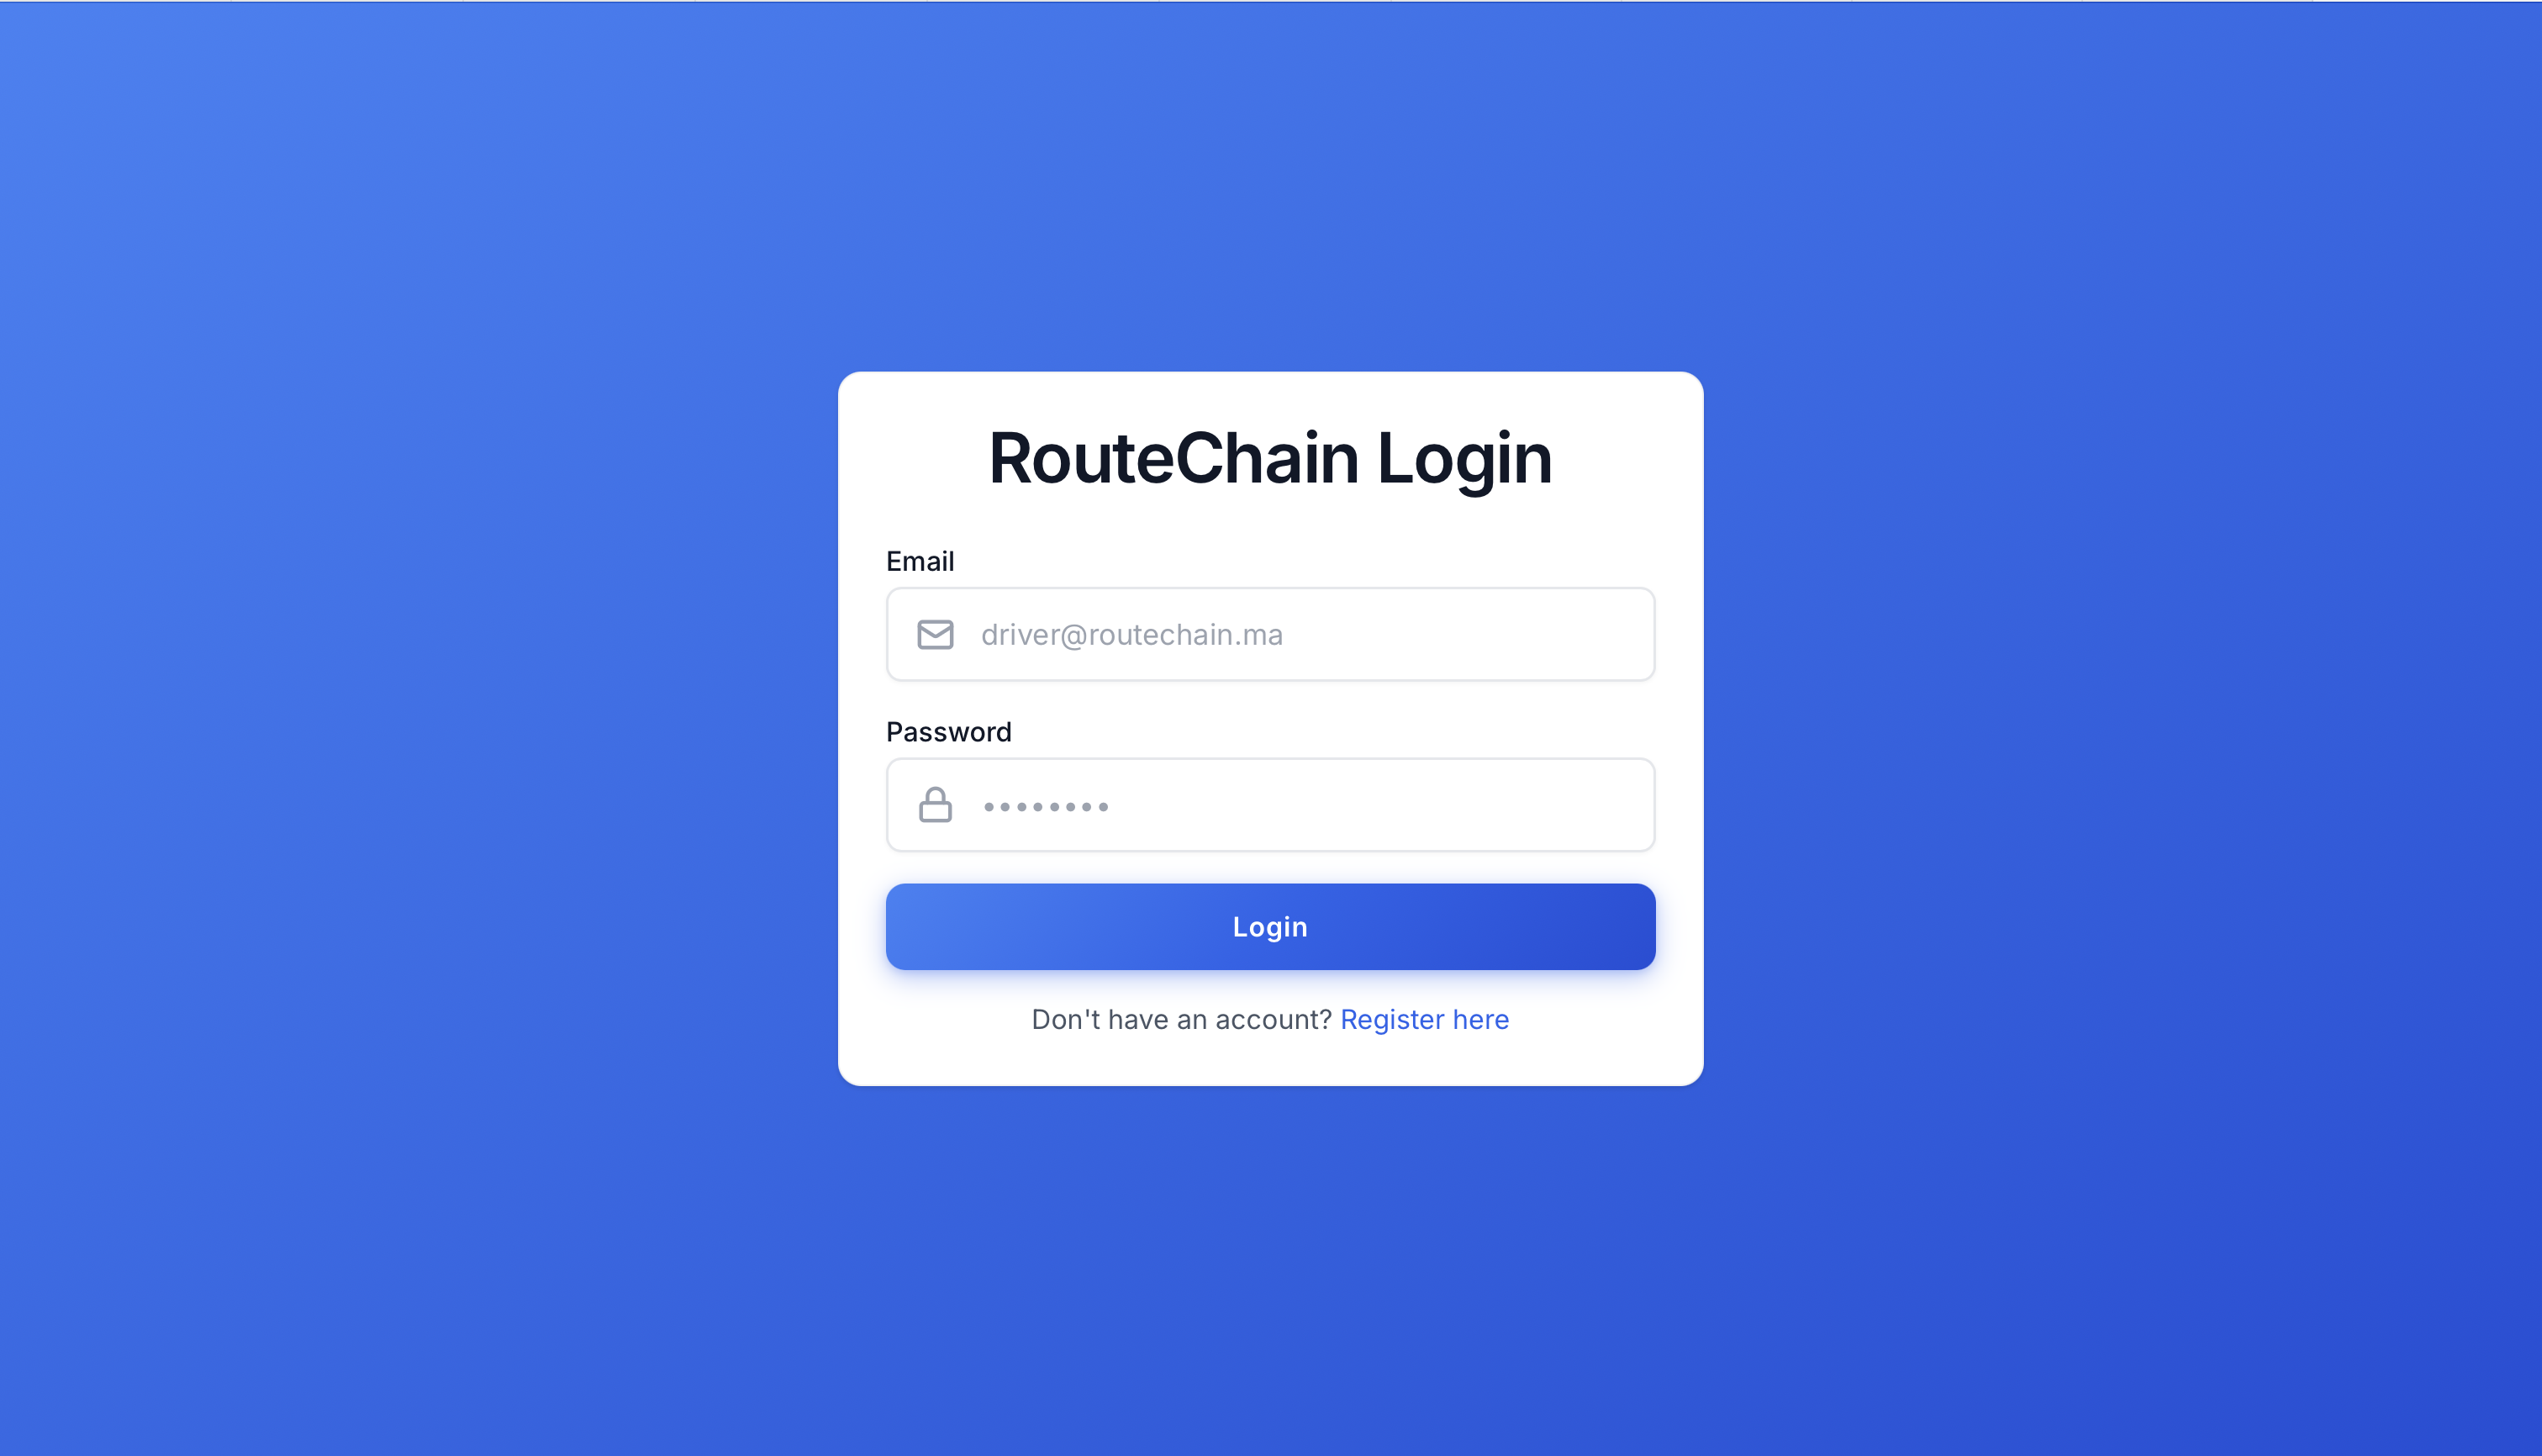
\includegraphics[width=0.92\textwidth]{resultats/login.png}
\caption{Page de connexion de l'application RouteChain}
\label{fig:screen_login}
\end{figure}

Le formulaire d'inscription permet la création d'un nouveau compte chauffeur avec validation en temps réel des champs. L'interface guide l'utilisateur à travers les informations requises : nom complet, adresse email, mot de passe avec indicateur de force, numéro de téléphone au format marocain, type de véhicule (moto, voiture, van, camion) et capacité maximale de colis. Cette conception assure que les données des chauffeurs sont complètes dès leur inscription.

\begin{figure}[H]
\centering
\includegraphics[width=0.92\textwidth]{resultats/register.png}
\caption{Page d'inscription avec formulaire de création de compte chauffeur}
\label{fig:screen_register}
\end{figure}

\subsection{Dashboard et Gestion des Tournées}

Le tableau de bord principal constitue le point d'entrée après connexion. Il affiche une vue d'ensemble des tournées du chauffeur avec des indicateurs clés : nombre de tournées actives, tournées complétées aujourd'hui, et distance totale parcourue. Chaque tournée est représentée sous forme de carte avec son nom, statut (planifiée, en cours, complétée), distance totale et nombre de points de livraison. Des boutons d'accès rapide permettent de créer une nouvelle tournée, gérer les clients et consulter les dépôts.

\begin{figure}[H]
\centering
\includegraphics[width=0.92\textwidth]{resultats/dashboard.png}
\caption{Dashboard principal affichant la liste des tournées}
\label{fig:screen_dashboard}
\end{figure}

\subsection{Création de Tournée}

L'interface de création de tournée est le cœur fonctionnel de l'application. Elle se divise en trois sections principales : les informations de la tournée (nom), la sélection du dépôt de départ, et l'ajout des points de livraison. L'utilisateur peut soit sélectionner un dépôt préexistant dans la base de données, soit saisir manuellement une adresse. Le géocodage automatique via l'API Nominatim (OpenStreetMap) convertit instantanément les adresses textuelles en coordonnées GPS précises.

\begin{figure}[H]
\centering
\includegraphics[width=0.92\textwidth]{resultats/create_route1.png}
\caption{Formulaire de création de tournée - Section dépôt et informations}
\label{fig:screen_route_form1}
\end{figure}

La section des points de livraison permet d'ajouter entre 1 et 20 destinations. Pour chaque point, l'utilisateur peut soit sélectionner un client existant (qui remplit automatiquement les coordonnées), soit saisir un nouveau client avec son nom, téléphone, adresse et instructions de livraison. Une prévisualisation cartographique interactive affiche en temps réel tous les points sur une carte Leaflet, permettant de valider visuellement les positions avant l'optimisation.

\begin{figure}[H]
\centering
\includegraphics[width=0.92\textwidth]{resultats/create_route2.png}
\caption{Formulaire de création de tournée - Points de livraison et carte}
\label{fig:screen_route_form2}
\end{figure}

\subsection{Détail de Tournée et Visualisation Cartographique}

La page de détail présente toutes les informations d'une tournée optimisée. Elle affiche la liste ordonnée des points de livraison selon l'ordre optimal calculé par Google OR-Tools, avec pour chaque point : le nom du client, l'adresse, le numéro de séquence et le statut de livraison. Les statistiques globales incluent la distance totale, le temps estimé et le nombre de colis. Des boutons d'action permettent de démarrer la tournée, confirmer les livraisons et exporter les données.

\begin{figure}[H]
\centering
\includegraphics[width=0.92\textwidth]{resultats/route_details1.png}
\caption{Page de détail d'une tournée avec informations et carte}
\label{fig:screen_route_detail1}
\end{figure}

La carte interactive affiche l'itinéraire optimisé avec des marqueurs numérotés pour chaque point de livraison. Le tracé polyline suit les routes réelles grâce à l'API OpenRouteService, offrant une visualisation précise du parcours. L'interface affiche également les informations de traçabilité blockchain : hash de transaction, numéro de bloc et horodatage d'enregistrement. Le bouton de vérification permet de contrôler l'intégrité des données en comparant le hash stocké avec celui recalculé.

\begin{figure}[H]
\centering
\includegraphics[width=0.92\textwidth]{resultats/route_details2.png}
\caption{Visualisation cartographique et informations blockchain}
\label{fig:screen_route_detail2}
\end{figure}

\subsection{Profil Utilisateur}

La page de profil permet au chauffeur de consulter et modifier ses informations personnelles. Elle affiche le nom complet, l'adresse email, le numéro de téléphone, le type de véhicule utilisé et la plaque d'immatriculation. Des statistiques de performance sont également présentées : nombre total de tournées effectuées, distance cumulée parcourue et taux de complétion. L'utilisateur peut mettre à jour ses informations via un formulaire d'édition accessible.

\begin{figure}[H]
\centering
\includegraphics[width=0.88\textwidth]{resultats/profile.png}
\caption{Page de profil du chauffeur avec informations personnelles}
\label{fig:screen_profile}
\end{figure}

\subsection{Gestion des Clients}

L'interface de gestion des clients offre une vue complète de la base de données clients. Elle présente la liste des clients enregistrés avec leurs coordonnées : nom, email, téléphone, entreprise et adresse. Une barre de recherche permet de filtrer rapidement les clients par nom ou email. Le formulaire d'ajout intègre le géocodage automatique pour convertir les adresses en coordonnées GPS, facilitant l'ajout de nouveaux clients lors de la création de tournées.

\begin{figure}[H]
\centering
\includegraphics[width=0.88\textwidth]{resultats/customers.png}
\caption{Interface de gestion des clients avec recherche et géocodage}
\label{fig:screen_customers}
\end{figure}

\subsection{Gestion des Dépôts}

La gestion des dépôts permet de définir les points de départ des tournées. L'interface affiche les dépôts enregistrés sous forme de cartes avec leur nom, adresse, coordonnées GPS et horaires d'ouverture. Un dépôt peut être marqué comme défaut pour la sélection automatique lors de la création de tournées. Le formulaire d'ajout inclut le géocodage automatique via Nominatim, permettant de convertir une adresse textuelle en latitude/longitude précises.

\begin{figure}[H]
\centering
\includegraphics[width=0.9\textwidth]{resultats/depots.png}
\caption{Interface de gestion des dépôts avec géocodage automatique}
\label{fig:screen_depots}
\end{figure}

\subsection{Panel Administrateur}

Le panel administrateur est réservé aux utilisateurs disposant du rôle admin. Il offre une vue d'ensemble de tous les chauffeurs enregistrés dans le système avec leurs informations : nom, email, type de véhicule et rôle actuel. L'administrateur peut modifier les rôles des utilisateurs (promotion en admin ou rétrogradation en driver), consulter l'historique complet des tournées de chaque chauffeur et gérer les accès au système.

\begin{figure}[H]
\centering
\includegraphics[width=0.9\textwidth]{resultats/admin_panel.png}
\caption{Panel d'administration avec gestion des chauffeurs}
\label{fig:screen_admin}
\end{figure}

\subsection{Dashboard Analytique}

Le tableau de bord analytique présente des indicateurs clés de performance (KPI) sous forme de visualisations graphiques. Il affiche le nombre total de tournées effectuées, la distance totale parcourue, le nombre de livraisons complétées et le taux de complétion moyen. Des graphiques d'évolution temporelle permettent d'analyser les tendances sur différentes périodes. Cette interface aide les gestionnaires à évaluer l'efficacité des opérations de livraison.

\begin{figure}[H]
\centering
\includegraphics[width=0.95\textwidth]{resultats/analytics_dash.png}
\caption{Tableau de bord analytique avec indicateurs de performance}
\label{fig:screen_analytics}
\end{figure}

%---------------------------------------------------------------------
\section{Conclusion}
%---------------------------------------------------------------------

Ce chapitre a présenté les technologies utilisées pour le développement de RouteChain. Chaque choix technologique a été justifié en fonction des besoins spécifiques du projet : performance pour FastAPI, flexibilité pour MongoDB, puissance d'optimisation pour OR-Tools, et traçabilité pour Ganache/Ethereum.

L'architecture modulaire et les technologies modernes sélectionnées garantissent la maintenabilité et l'évolutivité du système. Le chapitre suivant proposera une discussion sur les défis rencontrés et l'évaluation du système.



% Chapitre 5 : Discussion et Évaluation
%=====================================================================
%            CHAPITRE 5 : DISCUSSION ET ÉVALUATION
%=====================================================================

\chapter{Discussion et Évaluation}

%---------------------------------------------------------------------
\section{Introduction}
%---------------------------------------------------------------------

Ce chapitre propose une analyse critique du projet RouteChain. Nous examinerons les défis techniques rencontrés durant le développement, les stratégies adoptées pour la gestion des données, ainsi qu'une évaluation globale du système. Nous conclurons par une discussion sur les limitations actuelles et les perspectives d'évolution.

%---------------------------------------------------------------------
\section{Défis Techniques Rencontrés}
%---------------------------------------------------------------------

\subsection{Latence de l'Optimisation VRP}

L'un des premiers défis rencontrés concerne le temps de calcul de l'algorithme d'optimisation VRP. Pour des tournées comportant un grand nombre de points de livraison (au-delà de 20 points), le temps de réponse pouvait dépasser les attentes utilisateur.

\textbf{Solutions mises en œuvre :}
\begin{itemize}[leftmargin=2cm]
    \item Limitation du temps d'exécution du solveur OR-Tools à 30 secondes maximum
    \item Utilisation de la stratégie \texttt{PATH\_CHEAPEST\_ARC} pour obtenir rapidement une solution initiale
    \item Affichage d'un indicateur de progression pendant le calcul
\end{itemize}

\subsection{Coûts de Gas et Délais Blockchain}

L'interaction avec la blockchain Ethereum, même en environnement local (Ganache), introduit des contraintes spécifiques liées aux transactions.

\textbf{Problématiques identifiées :}
\begin{itemize}[leftmargin=2cm]
    \item Chaque transaction blockchain consomme du "gas" (unité de coût computationnel)
    \item Les transactions nécessitent un temps de confirmation
    \item En cas d'erreur, les transactions échouées consomment quand même du gas
\end{itemize}

\textbf{Optimisations réalisées :}
\begin{itemize}[leftmargin=2cm]
    \item Stockage uniquement du hash des données (32 bytes) plutôt que des données complètes
    \item Mode dégradé permettant le fonctionnement sans blockchain disponible
    \item Gestion des erreurs avec retry automatique
\end{itemize}

\subsection{Synchronisation MongoDB - Blockchain}

Un défi architectural majeur réside dans la synchronisation entre les données stockées dans MongoDB et les enregistrements blockchain.

\textbf{Stratégie adoptée :}
\begin{itemize}[leftmargin=2cm]
    \item MongoDB reste la source principale des données détaillées
    \item La blockchain stocke uniquement les hash et métadonnées critiques
    \item Les informations de transaction (hash, bloc) sont enregistrées dans MongoDB pour référence
\end{itemize}

% \subsection{Gestion du CORS pour l'Accès Mobile}

% L'accès à l'application depuis des appareils mobiles sur le même réseau local a nécessité une configuration particulière du CORS (Cross-Origin Resource Sharing).

% \textbf{Solution :}
% \begin{itemize}[leftmargin=2cm]
%     \item Configuration du backend pour accepter toutes les origines en développement
%     \item Détection automatique de l'URL de l'API basée sur le hostname d'accès
%     \item Documentation claire pour le déploiement en production avec des origines spécifiques
% \end{itemize}

%---------------------------------------------------------------------
\section{Gestion des Données et Intégrité}
%---------------------------------------------------------------------

\subsection{Mécanisme de Vérification par Hash}

Le système de vérification d'intégrité repose sur le calcul d'un hash SHA-256 des données immuables d'une tournée.

\begin{table}[H]
\centering
\caption{Données incluses dans le calcul du hash}
\begin{tabular}{|l|l|}
\hline
\textbf{Champ} & \textbf{Justification} \\
\hline
route\_id & Identifiant unique de la tournée \\
route\_name & Nom donné par l'utilisateur \\
depot\_location & Coordonnées du point de départ \\
delivery\_points (adresses et coordonnées) & Définition des livraisons \\
\hline
\end{tabular}
\end{table}

\textbf{Important :} Les champs mutables (statut, horodatages, livraisons confirmées) sont exclus du calcul du hash pour permettre les mises à jour légitimes sans invalider la vérification.

\subsection{Distinction entre Données Mutables et Immuables}

\begin{table}[H]
\centering
\caption{Classification des données de tournée}
\begin{tabular}{|l|l|l|}
\hline
\textbf{Catégorie} & \textbf{Exemples} & \textbf{Traitement} \\
\hline
Immuables & route\_id, points de livraison, dépôt & Inclus dans le hash blockchain \\
\hline
Mutables & status, completed\_at, confirmations & Exclus du hash, mis à jour librement \\
\hline
\end{tabular}
\end{table}

Cette distinction permet de garantir que les données fondamentales de la tournée (qui l'a créée, où sont les livraisons) restent vérifiables, tout en autorisant l'évolution normale du statut d'exécution.

%---------------------------------------------------------------------
% \section{Évaluation du Système}
% %---------------------------------------------------------------------

% \subsection{Tests Fonctionnels}

% L'ensemble des fonctionnalités définies dans le cahier des charges ont été implémentées et testées.

% \begin{table}[H]
% \centering
% \caption{Couverture des exigences fonctionnelles}
% \begin{tabular}{|l|c|c|}
% \hline
% \textbf{Module} & \textbf{Exigences} & \textbf{Implémentées} \\
% \hline
% Authentification & 5 & 5 (100\%) \\
% Gestion des rôles & 3 & 3 (100\%) \\
% Clients et Dépôts & 5 & 5 (100\%) \\
% Tournées & 6 & 6 (100\%) \\
% Exécution & 5 & 5 (100\%) \\
% Blockchain & 5 & 5 (100\%) \\
% Analytique & 4 & 4 (100\%) \\
% \hline
% \textbf{Total} & \textbf{33} & \textbf{33 (100\%)} \\
% \hline
% \end{tabular}
% \end{table}

% \subsection{Métriques de Performance}

% \begin{table}[H]
% \centering
% \caption{Métriques de performance mesurées}
% \begin{tabular}{|l|l|l|}
% \hline
% \textbf{Métrique} & \textbf{Valeur mesurée} & \textbf{Objectif} \\
% \hline
% Temps de réponse API (opérations courantes) & < 300 ms & < 500 ms \\
% \hline
% Temps d'optimisation VRP (10 points) & 2-3 secondes & < 10 secondes \\
% \hline
% Temps d'optimisation VRP (20 points) & 5-8 secondes & < 10 secondes \\
% \hline
% Confirmation transaction blockchain & 1-2 secondes & N/A (Ganache) \\
% \hline
% Chargement initial de l'application & < 2 secondes & < 3 secondes \\
% \hline
% \end{tabular}
% \end{table}

% \subsection{Retours Utilisateurs}

% Des tests d'acceptation ont été réalisés avec des utilisateurs potentiels. Les principaux retours sont :

% \textbf{Points positifs :}
% \begin{itemize}[leftmargin=2cm]
%     \item Interface intuitive et moderne
%     \item Visualisation cartographique claire
%     \item Rapidité de l'optimisation
%     \item Concept innovant de la traçabilité blockchain
% \end{itemize}

% \textbf{Points d'amélioration identifiés :}
% \begin{itemize}[leftmargin=2cm]
%     \item Ajout d'une application mobile native pour les chauffeurs
%     \item Intégration avec des systèmes GPS temps réel
%     \item Export vers d'autres formats (Excel, KML)
% \end{itemize}

%---------------------------------------------------------------------
% Section déplacée vers Conclusion Générale
%---------------------------------------------------------------------
% \section{Limitations et Perspectives}
% %---------------------------------------------------------------------

% \subsection{Limitations Actuelles}

% \begin{enumerate}[leftmargin=2cm]
%     \item \textbf{Blockchain locale :} L'utilisation de Ganache limite la solution à un environnement de développement. Un déploiement sur un testnet ou mainnet Ethereum nécessiterait une gestion des coûts de gas réels.
    
%     \item \textbf{Scalabilité VRP :} Pour des flottes avec plusieurs véhicules ou des centaines de points, l'algorithme actuel devrait être optimisé ou distribué.
    
%     \item \textbf{Absence de temps réel :} Le système ne propose pas de suivi GPS en temps réel des véhicules.
    
%     \item \textbf{Dépendance aux APIs externes :} Le fonctionnement optimal dépend de la disponibilité d'OpenRouteService et Nominatim.
% \end{enumerate}

% \subsection{Perspectives d'Évolution}

% \begin{enumerate}[leftmargin=2cm]
%     \item \textbf{Déploiement sur Blockchain publique :} Migration vers un testnet Ethereum (Sepolia, Goerli) puis vers le mainnet pour une utilisation en production.
    
%     \item \textbf{Application mobile native :} Développement d'une application Flutter ou React Native dédiée aux chauffeurs avec GPS intégré.
    
%     \item \textbf{Intelligence artificielle :} Intégration de modèles de machine learning pour la prédiction des temps de livraison et l'optimisation dynamique.
    
%     \item \textbf{Multi-véhicules :} Extension du solveur VRP pour gérer des flottes de plusieurs véhicules avec contraintes de capacité.
    
%     \item \textbf{Intégration ERP :} Connecteurs pour les systèmes de gestion d'entreprise (SAP, Odoo, etc.).
% \end{enumerate}

%---------------------------------------------------------------------
\section{Conclusion}
%---------------------------------------------------------------------

Ce chapitre a permis d'analyser en profondeur les défis techniques rencontrés lors du développement de RouteChain et les solutions adoptées. L'évaluation du système montre une couverture complète des exigences fonctionnelles avec des performances satisfaisantes.

Les limitations identifiées, principalement liées à l'environnement de développement (blockchain locale) et à la scalabilité, ouvrent des perspectives d'évolution intéressantes pour transformer RouteChain en une solution de production complète.

Le système actuel constitue une preuve de concept fonctionnelle démontrant la faisabilité et l'intérêt de combiner optimisation VRP et traçabilité blockchain dans le domaine de la logistique du dernier kilomètre.


% Conclusion Générale
%=====================================================================
%                    CONCLUSION GÉNÉRALE
%=====================================================================

\chapter*{Conclusion Générale}
\addcontentsline{toc}{chapter}{Conclusion Générale}
\markboth{Conclusion Générale}{Conclusion Générale}

\vspace{1cm}

Le projet RouteChain, présenté dans ce rapport, constitue une contribution significative à l'intersection de deux domaines technologiques majeurs : l'optimisation combinatoire appliquée à la logistique et la technologie Blockchain pour la garantie d'intégrité des données. Face aux défis croissants de la logistique du dernier kilomètre, exacerbés par l'explosion du commerce électronique, nous avons développé une solution complète permettant aux entreprises de livraison d'optimiser leurs tournées tout en garantissant une traçabilité irréfutable de leurs opérations.

L'application développée répond pleinement aux objectifs initialement fixés. L'intégration de Google OR-Tools permet de calculer des séquences de livraison optimales, réduisant significativement les distances parcourues et les temps de trajet. Le smart contract RouteRegistry, déployé sur Ethereum, assure l'enregistrement immuable des données de chaque tournée, offrant une preuve vérifiable de l'intégrité des informations. L'interface utilisateur moderne, développée avec React et Tailwind CSS, offre une expérience fluide tant sur desktop que sur mobile. Enfin, l'architecture évolutive basée sur FastAPI et MongoDB garantit la maintenabilité et l'extensibilité du système.

D'un point de vue technique, ce projet nous a permis d'approfondir nos compétences dans plusieurs domaines : le développement full-stack avec des frameworks modernes, la résolution de problèmes d'optimisation combinatoire, et le développement de smart contracts pour la blockchain Ethereum.

Cependant, la solution actuelle présente certaines limitations qu'il convient de mentionner. L'utilisation de Ganache comme blockchain locale limite le déploiement à un environnement de développement, car un passage vers un testnet ou mainnet Ethereum nécessiterait une gestion des coûts de gas réels. L'algorithme VRP implémenté, bien que performant pour des tournées de taille moyenne, devrait être optimisé ou distribué pour gérer des flottes multi-véhicules ou des centaines de points de livraison. Par ailleurs, le système ne propose pas de suivi GPS en temps réel des véhicules, et son fonctionnement optimal dépend de la disponibilité des APIs externes OpenRouteService et Nominatim.

Ces limitations ouvrent néanmoins des perspectives d'évolution prometteuses. Le déploiement sur une blockchain publique, en commençant par un testnet Ethereum comme Sepolia avant d'envisager le mainnet, constitue une première étape vers une solution de production. Le développement d'une application mobile native avec Flutter ou React Native, intégrant le GPS du smartphone, améliorerait considérablement l'expérience des chauffeurs sur le terrain. L'intégration de modèles de machine learning pour la prédiction des temps de livraison et l'optimisation dynamique représente une piste d'amélioration significative. L'extension du solveur VRP pour gérer des flottes multi-véhicules avec contraintes de capacité élargirait le champ d'application de la solution. Enfin, le développement de connecteurs pour les systèmes de gestion d'entreprise (SAP, Odoo) faciliterait l'intégration dans les écosystèmes existants.

En définitive, RouteChain démontre la faisabilité et la pertinence de combiner optimisation algorithmique et technologie blockchain pour répondre aux enjeux contemporains de la logistique. Cette approche hybride, alliant efficacité opérationnelle et transparence des données, représente une voie d'avenir pour le secteur de la livraison du dernier kilomètre.


\newpage

\nocite{*}
\bibliographystyle{plain}
\bibliography{references.bib}

\end{document}
